%% bare_jrnl.tex
%% V1.4b
%% 2015/08/26
%% by Michael Shell
%% see http://www.michaelshell.org/
%% for current contact information.
%%
%% This is a skeleton file demonstrating the use of IEEEtran.cls
%% (requires IEEEtran.cls version 1.8b or later) with an IEEE
%% journal paper.
%%
%% Support sites:
%% http://www.michaelshell.org/tex/ieeetran/
%% http://www.ctan.org/pkg/ieeetran
%% and
%% http://www.ieee.org/

%%*************************************************************************
%% Legal Notice:
%% This code is offered as-is without any warranty either expressed or
%% implied; without even the implied warranty of MERCHANTABILITY or
%% FITNESS FOR A PARTICULAR PURPOSE!
%% User assumes all risk.
%% In no event shall the IEEE or any contributor to this code be liable for
%% any damages or losses, including, but not limited to, incidental,
%% consequential, or any other damages, resulting from the use or misuse
%% of any information contained here.
%%
%% All comments are the opinions of their respective authors and are not
%% necessarily endorsed by the IEEE.
%%
%% This work is distributed under the LaTeX Project Public License (LPPL)
%% ( http://www.latex-project.org/ ) version 1.3, and may be freely used,
%% distributed and modified. A copy of the LPPL, version 1.3, is included
%% in the base LaTeX documentation of all distributions of LaTeX released
%% 2003/12/01 or later.
%% Retain all contribution notices and credits.
%% ** Modified files should be clearly indicated as such, including  **
%% ** renaming them and changing author support contact information. **
%%*************************************************************************


% *** Authors should verify (and, if needed, correct) their LaTeX system  ***
% *** with the testflow diagnostic prior to trusting their LaTeX platform ***
% *** with production work. The IEEE's font choices and paper sizes can   ***
% *** trigger bugs that do not appear when using other class files.       ***                          ***
% The testflow support page is at:
% http://www.michaelshell.org/tex/testflow/



\documentclass[journal]{IEEEtran}
%
% If IEEEtran.cls has not been installed into the LaTeX system files,
% manually specify the path to it like:
% \documentclass[journal]{../sty/IEEEtran}





% Some very useful LaTeX packages include:
% (uncomment the ones you want to load)


% *** MISC UTILITY PACKAGES ***
%
%\usepackage{ifpdf}
% Heiko Oberdiek's ifpdf.sty is very useful if you need conditional
% compilation based on whether the output is pdf or dvi.
% usage:
% \ifpdf
%   % pdf code
% \else
%   % dvi code
% \fi
% The latest version of ifpdf.sty can be obtained from:
% http://www.ctan.org/pkg/ifpdf
% Also, note that IEEEtran.cls V1.7 and later provides a builtin
% \ifCLASSINFOpdf conditional that works the same way.
% When switching from latex to pdflatex and vice-versa, the compiler may
% have to be run twice to clear warning/error messages.






% *** CITATION PACKAGES ***
%
%\usepackage{cite}
% cite.sty was written by Donald Arseneau
% V1.6 and later of IEEEtran pre-defines the format of the cite.sty package
% \cite{} output to follow that of the IEEE. Loading the cite package will
% result in citation numbers being automatically sorted and properly
% "compressed/ranged". e.g., [1], [9], [2], [7], [5], [6] without using
% cite.sty will become [1], [2], [5]--[7], [9] using cite.sty. cite.sty's
% \cite will automatically add leading space, if needed. Use cite.sty's
% noadjust option (cite.sty V3.8 and later) if you want to turn this off
% such as if a citation ever needs to be enclosed in parenthesis.
% cite.sty is already installed on most LaTeX systems. Be sure and use
% version 5.0 (2009-03-20) and later if using hyperref.sty.
% The latest version can be obtained at:
% http://www.ctan.org/pkg/cite
% The documentation is contained in the cite.sty file itself.






% *** GRAPHICS RELATED PACKAGES ***
%
\ifCLASSINFOpdf
  % \usepackage[pdftex]{graphicx}
  % declare the path(s) where your graphic files are
  % \graphicspath{{../pdf/}{../jpeg/}}
  % and their extensions so you won't have to specify these with
  % every instance of \includegraphics
  % \DeclareGraphicsExtensions{.pdf,.jpeg,.png}
\else
  % or other class option (dvipsone, dvipdf, if not using dvips). graphicx
  % will default to the driver specified in the system graphics.cfg if no
  % driver is specified.
  % \usepackage[dvips]{graphicx}
  % declare the path(s) where your graphic files are
  % \graphicspath{{../eps/}}
  % and their extensions so you won't have to specify these with
  % every instance of \includegraphics
  % \DeclareGraphicsExtensions{.eps}
\fi
% graphicx was written by David Carlisle and Sebastian Rahtz. It is
% required if you want graphics, photos, etc. graphicx.sty is already
% installed on most LaTeX systems. The latest version and documentation
% can be obtained at:
% http://www.ctan.org/pkg/graphicx
% Another good source of documentation is "Using Imported Graphics in
% LaTeX2e" by Keith Reckdahl which can be found at:
% http://www.ctan.org/pkg/epslatex
%
% latex, and pdflatex in dvi mode, support graphics in encapsulated
% postscript (.eps) format. pdflatex in pdf mode supports graphics
% in .pdf, .jpeg, .png and .mps (metapost) formats. Users should ensure
% that all non-photo figures use a vector format (.eps, .pdf, .mps) and
% not a bitmapped formats (.jpeg, .png). The IEEE frowns on bitmapped formats
% which can result in "jaggedy"/blurry rendering of lines and letters as
% well as large increases in file sizes.
%
% You can find documentation about the pdfTeX application at:
% http://www.tug.org/applications/pdftex





% *** MATH PACKAGES ***
%
%\usepackage{amsmath}
% A popular package from the American Mathematical Society that provides
% many useful and powerful commands for dealing with mathematics.
%
% Note that the amsmath package sets \interdisplaylinepenalty to 10000
% thus preventing page breaks from occurring within multiline equations. Use:
%\interdisplaylinepenalty=2500
% after loading amsmath to restore such page breaks as IEEEtran.cls normally
% does. amsmath.sty is already installed on most LaTeX systems. The latest
% version and documentation can be obtained at:
% http://www.ctan.org/pkg/amsmath





% *** SPECIALIZED LIST PACKAGES ***
%
%\usepackage{algorithmic}
% algorithmic.sty was written by Peter Williams and Rogerio Brito.
% This package provides an algorithmic environment fo describing algorithms.
% You can use the algorithmic environment in-text or within a figure
% environment to provide for a floating algorithm. Do NOT use the algorithm
% floating environment provided by algorithm.sty (by the same authors) or
% algorithm2e.sty (by Christophe Fiorio) as the IEEE does not use dedicated
% algorithm float types and packages that provide these will not provide
% correct IEEE style captions. The latest version and documentation of
% algorithmic.sty can be obtained at:
% http://www.ctan.org/pkg/algorithms
% Also of interest may be the (relatively newer and more customizable)
% algorithmicx.sty package by Szasz Janos:
% http://www.ctan.org/pkg/algorithmicx
\usepackage{booktabs}   % For professional-quality lines
\usepackage{tabularx}   % For tables that fit the page width
\usepackage{graphicx}




% *** ALIGNMENT PACKAGES ***
%
%\usepackage{array}
% Frank Mittelbach's and David Carlisle's array.sty patches and improves
% the standard LaTeX2e array and tabular environments to provide better
% appearance and additional user controls. As the default LaTeX2e table
% generation code is lacking to the point of almost being broken with
% respect to the quality of the end results, all users are strongly
% advised to use an enhanced (at the very least that provided by array.sty)
% set of table tools. array.sty is already installed on most systems. The
% latest version and documentation can be obtained at:
% http://www.ctan.org/pkg/array


% IEEEtran contains the IEEEeqnarray family of commands that can be used to
% generate multiline equations as well as matrices, tables, etc., of high
% quality.




% *** SUBFIGURE PACKAGES ***
%\ifCLASSOPTIONcompsoc
%  \usepackage[caption=false,font=normalsize,labelfont=sf,textfont=sf]{subfig}
%\else
%  \usepackage[caption=false,font=footnotesize]{subfig}
%\fi
% subfig.sty, written by Steven Douglas Cochran, is the modern replacement
% for subfigure.sty, the latter of which is no longer maintained and is
% incompatible with some LaTeX packages including fixltx2e. However,
% subfig.sty requires and automatically loads Axel Sommerfeldt's caption.sty
% which will override IEEEtran.cls' handling of captions and this will result
% in non-IEEE style figure/table captions. To prevent this problem, be sure
% and invoke subfig.sty's "caption=false" package option (available since
% subfig.sty version 1.3, 2005/06/28) as this is will preserve IEEEtran.cls
% handling of captions.
% Note that the Computer Society format requires a larger sans serif font
% than the serif footnote size font used in traditional IEEE formatting
% and thus the need to invoke different subfig.sty package options depending
% on whether compsoc mode has been enabled.
%
% The latest version and documentation of subfig.sty can be obtained at:
% http://www.ctan.org/pkg/subfig




% *** FLOAT PACKAGES ***
%
%\usepackage{fixltx2e}
% fixltx2e, the successor to the earlier fix2col.sty, was written by
% Frank Mittelbach and David Carlisle. This package corrects a few problems
% in the LaTeX2e kernel, the most notable of which is that in current
% LaTeX2e releases, the ordering of single and double column floats is not
% guaranteed to be preserved. Thus, an unpatched LaTeX2e can allow a
% single column figure to be placed prior to an earlier double column
% figure.
% Be aware that LaTeX2e kernels dated 2015 and later have fixltx2e.sty's
% corrections already built into the system in which case a warning will
% be issued if an attempt is made to load fixltx2e.sty as it is no longer
% needed.
% The latest version and documentation can be found at:
% http://www.ctan.org/pkg/fixltx2e


%\usepackage{stfloats}
% stfloats.sty was written by Sigitas Tolusis. This package gives LaTeX2e
% the ability to do double column floats at the bottom of the page as well
% as the top. (e.g., "\begin{figure*}[!b]" is not normally possible in
% LaTeX2e). It also provides a command:
%\fnbelowfloat
% to enable the placement of footnotes below bottom floats (the standard
% LaTeX2e kernel puts them above bottom floats). This is an invasive package
% which rewrites many portions of the LaTeX2e float routines. It may not work
% with other packages that modify the LaTeX2e float routines. The latest
% version and documentation can be obtained at:
% http://www.ctan.org/pkg/stfloats
% Do not use the stfloats baselinefloat ability as the IEEE does not allow
% \baselineskip to stretch. Authors submitting work to the IEEE should note
% that the IEEE rarely uses double column equations and that authors should try
% to avoid such use. Do not be tempted to use the cuted.sty or midfloat.sty
% packages (also by Sigitas Tolusis) as the IEEE does not format its papers in
% such ways.
% Do not attempt to use stfloats with fixltx2e as they are incompatible.
% Instead, use Morten Hogholm'a dblfloatfix which combines the features
% of both fixltx2e and stfloats:
%
% \usepackage{dblfloatfix}
% The latest version can be found at:
% http://www.ctan.org/pkg/dblfloatfix




%\ifCLASSOPTIONcaptionsoff
%  \usepackage[nomarkers]{endfloat}
% \let\MYoriglatexcaption\caption
% \renewcommand{\caption}[2][\relax]{\MYoriglatexcaption[#2]{#2}}
%\fi
% endfloat.sty was written by James Darrell McCauley, Jeff Goldberg and
% Axel Sommerfeldt. This package may be useful when used in conjunction with
% IEEEtran.cls'  captionsoff option. Some IEEE journals/societies require that
% submissions have lists of figures/tables at the end of the paper and that
% figures/tables without any captions are placed on a page by themselves at
% the end of the document. If needed, the draftcls IEEEtran class option or
% \CLASSINPUTbaselinestretch interface can be used to increase the line
% spacing as well. Be sure and use the nomarkers option of endfloat to
% prevent endfloat from "marking" where the figures would have been placed
% in the text. The two hack lines of code above are a slight modification of
% that suggested by in the endfloat docs (section 8.4.1) to ensure that
% the full captions always appear in the list of figures/tables - even if
% the user used the short optional argument of \caption[]{}.
% IEEE papers do not typically make use of \caption[]'s optional argument,
% so this should not be an issue. A similar trick can be used to disable
% captions of packages such as subfig.sty that lack options to turn off
% the subcaptions:
% For subfig.sty:
% \let\MYorigsubfloat\subfloat
% \renewcommand{\subfloat}[2][\relax]{\MYorigsubfloat[]{#2}}
% However, the above trick will not work if both optional arguments of
% the \subfloat command are used. Furthermore, there needs to be a
% description of each subfigure *somewhere* and endfloat does not add
% subfigure captions to its list of figures. Thus, the best approach is to
% avoid the use of subfigure captions (many IEEE journals avoid them anyway)
% and instead reference/explain all the subfigures within the main caption.
% The latest version of endfloat.sty and its documentation can obtained at:
% http://www.ctan.org/pkg/endfloat
%
% The IEEEtran \ifCLASSOPTIONcaptionsoff conditional can also be used
% later in the document, say, to conditionally put the References on a
% page by themselves.




% *** PDF, URL AND HYPERLINK PACKAGES ***
%
%\usepackage{url}
% url.sty was written by Donald Arseneau. It provides better support for
% handling and breaking URLs. url.sty is already installed on most LaTeX
% systems. The latest version and documentation can be obtained at:
% http://www.ctan.org/pkg/url
% Basically, \url{my_url_here}.




% *** Do not adjust lengths that control margins, column widths, etc. ***
% *** Do not use packages that alter fonts (such as pslatex).         ***
% There should be no need to do such things with IEEEtran.cls V1.6 and later.
% (Unless specifically asked to do so by the journal or conference you plan
% to submit to, of course. )


% correct bad hyphenation here
\hyphenation{op-tical net-works semi-conduc-tor}


\begin{document}
%
% paper title
% Titles are generally capitalized except for words such as a, an, and, as,
% at, but, by, for, in, nor, of, on, or, the, to and up, which are usually
% not capitalized unless they are the first or last word of the title.
% Linebreaks \\ can be used within to get better formatting as desired.
% Do not put math or special symbols in the title.
\title{Explainable and Adversarially Aware Detection of Enterprise Digital Sanitization Activity}
%
%
% author names and IEEE memberships
% note positions of commas and nonbreaking spaces ( ~ ) LaTeX will not break
% a structure at a ~ so this keeps an author's name from being broken across
% two lines.
% use \thanks{} to gain access to the first footnote area
% a separate \thanks must be used for each paragraph as LaTeX2e's \thanks
% was not built to handle multiple paragraphs
%

\author{\IEEEauthorblockN{Usang Usang Ibiang}
\IEEEauthorblockA{\textit{Computer Engineering Department} \\
\textit{University of Uyo, Nigeria}\\
sangy001@yahoo.com}
\and
\IEEEauthorblockN{Bliss Utibe-Abasi Stephen*}
\IEEEauthorblockA{\textit{Computer Engineering Department} \\
\textit{University of Uyo, Nigeria}\\
blissstephen@uniuyo.edu.ng}
\and
\IEEEauthorblockN{Oluseun Damilola Oyeleke}
\IEEEauthorblockA{\textit{Computer Engineering Department} \\
\textit{Nile University, Abuja, Nigeria}\\
contactseun@gmail.com}
\and
\IEEEauthorblockN{Agbaji Adai Samuel}
\IEEEauthorblockA{\textit{Computer Engineering Department} \\
\textit{University of Uyo, Nigeria}\\
agbasam@yahoo.com}
\and
\IEEEauthorblockN{Emmanuel Abraham Udoh}
\IEEEauthorblockA{\textit{Computer Engineering Department} \\
\textit{University of Uyo, Nigeria}\\
abrahamemmanuel085@gmail.com}
\and
\IEEEauthorblockN{Philip Asuquo}
\IEEEauthorblockA{\textit{Computer Engineering Department} \\
\textit{University of Uyo, Nigeria}\\
philipasuquo@uniuyo.edu.ng}
}

% note the % following the last \IEEEmembership and also \thanks -
% these prevent an unwanted space from occurring between the last author name
% and the end of the author line. i.e., if you had this:
%
% \author{....lastname \thanks{...} \thanks{...} }
%                     ^------------^------------^----Do not want these spaces!
%
% a space would be appended to the last name and could cause every name on that
% line to be shifted left slightly. This is one of those "LaTeX things". For
% instance, "\textbf{A} \textbf{B}" will typeset as "A B" not "AB". To get
% "AB" then you have to do: "\textbf{A}\textbf{B}"
% \thanks is no different in this regard, so shield the last } of each \thanks
% that ends a line with a % and do not let a space in before the next \thanks.
% Spaces after \IEEEmembership other than the last one are OK (and needed) as
% you are supposed to have spaces between the names. For what it is worth,
% this is a minor point as most people would not even notice if the said evil
% space somehow managed to creep in.



% The paper headers
\markboth{Journal of \LaTeX\ Class Files,~Vol.~14, No.~8, August~2015}{Emmanuel Abraham Udoh}
% The only time the second header will appear is for the odd numbered pages
% after the title page when using the twoside option.
%
% *** Note that you probably will NOT want to include the author's ***
% *** name in the headers of peer review papers.                   ***
% You can use \ifCLASSOPTIONpeerreview for conditional compilation here if
% you desire.












% If you want to put a publisher's ID mark on the page you can do it like
% this:
%\IEEEpubid{0000--0000/00\$00.00~\copyright~2015 IEEE}
% Remember, if you use this you must call \IEEEpubidadjcol in the second
% column for its text to clear the IEEEpubid mark.



% use for special paper notices
%\IEEEspecialpapernotice{(Invited Paper)}




% make the title area
\maketitle

% As a general rule, do not put math, special symbols or citations
% in the abstract or keywords.
\begin{abstract}
Enterprise environments generate authentication telemetry at a scale where malicious activity is rare, temporally clustered, and difficult to separate from legitimate use. This paper evaluates an explainable ensemble pipeline using LANL authentication events labeled from the accompanying red-team ground truth, group-aware validation, cross-validation, adversarial stress tests, ablation, and complexity measurements. At a threshold of 0.99237144 selected on a validation set and applied unchanged to the held-out test set, the meta-classifier obtained PR-AUC, macro-F1, and malicious recall of 1.0 with 0 false positives per 1000 events. These values are not evidence of generalizable behavioral detection: XGBoost assigned all feature importance to \texttt{hour\_cos}, its mean absolute SHAP value was 8.187043 while every other feature was 0, removal of the temporal feature group reduced PR-AUC to 0.208214, and the distribution-shift test reduced PR-AUC to 0.032199. The principal finding is therefore that conventional held-out evaluation can substantially overstate security-model capability when malicious and benign observations are separated by a temporal sampling artifact.
\end{abstract}

% Note that keywords are not normally used for peerreview papers.
\begin{IEEEkeywords}
Insider threat detection, digital sanitization, explainable artificial intelligence, adversarial machine learning, enterprise telemetry, graph analytics.
\end{IEEEkeywords}






% For peer review papers, you can put extra information on the cover
% page as needed:
% \ifCLASSOPTIONpeerreview
% \begin{center} \bfseries EDICS Category: 3-BBND \end{center}
% \fi
%
% For peerreview papers, this IEEEtran command inserts a page break and
% creates the second title. It will be ignored for other modes.
\IEEEpeerreviewmaketitle



\section{Introduction}
Insider threat detection remains a difficult security problem because the actor is already embedded within legitimate organizational workflows. Current literature characterizes insider detection as a setting shaped by sparse labels, behavioral heterogeneity, noisy event logs, and adaptive misuse patterns \cite{sarker2023insider,al2023review,liu2024graph}. Digital sanitization activity is especially difficult because wiping, deletion, removable-media use, path traversal, and authentication changes may be benign in isolation. Current trends therefore favor behavioral and contextual modeling that connects accounts, hosts, files, devices, and time rather than relying on isolated indicators of compromise \cite{al2023review,liu2024graph}.

Enterprise telemetry is large, noisy, and highly imbalanced, making sanitization-related insider activity difficult to detect at a usable operating point. A detector may assign meaningful risk scores while still missing malicious events when a fixed threshold is applied. This creates a practical challenge for security teams: they require high coverage, low alert volume, and interpretable evidence for analyst review, but these objectives often conflict under severe class imbalance.

Prior studies have advanced anomaly detection, supervised classification, sequence modeling, and graph-based insider analytics, but important gaps remain. Many approaches emphasize aggregate accuracy without sufficient attention to false positives per operational volume, malicious recall at selected thresholds, explanation stability, or adversarial low-and-slow behavior. In addition, fewer studies jointly evaluate temporal, entropy-based, peer-normalized, removable-media, and graph-centrality features within one explainable detection workflow.

The study is motivated by the operational need to identify rare sanitization-related events before they erase evidence, conceal misuse, or enable exfiltration. It is also motivated by the need for analyst-facing explanations that show why an event was scored as risky. Explainable and adversarially aware modeling offers an opportunity to connect detection performance with evidence that can support triage and governance \cite{ali2023xai,rosati2023blackbox}.

The objectives are: (i) to develop a model that detects enterprise digital sanitization activity from harmonized event telemetry; (ii) to evaluate tree-based, support-vector, deep-tabular, sequence, and meta-classification performance using precision--recall, macro-F1, malicious recall, and false-positive metrics; (iii) to quantify the contribution of temporal, peer-relative, graph, and event-sequence features; and (iv) to assess explanation behavior, adversarial robustness, and distribution shift.

The study contributes to security analytics by demonstrating how rare insider sanitization behavior must be evaluated as an operational and temporal-generalization problem rather than only as a classification benchmark. Its findings show why validation-selected thresholds, time-sensitive stress testing, ablation, and explanation diagnostics are necessary before apparently strong scores can support operational claims.

The contributions are threefold. First, the paper presents a feature design that links cyclic time, peer deviation, graph centrality, and event sequences. Second, it evaluates tree, support-vector, deep-tabular, sequence, and meta-classifier components using validation/test separation, five-fold group cross-validation, significance testing, ablation, robustness testing, and complexity measurement. Third, it reports an important negative result: near-perfect random-split performance was driven by a temporal proxy rather than by the intended behavioral features, demonstrating how naive evaluation can misrepresent capability in temporally clustered security data.

Section 2 reviews the literature on insider threat detection, graph analytics, explainability, and adversarial robustness. Section 3 describes the methodology and experimental design. Section 4 presents the results. Section 5 discusses operational implications, and Section 6 concludes the paper with the main numerical findings.

\section{Literature Review}
\subsection{Evolution of Insider Threat Detection Research}
\subsubsection{Reconstruction and Behavioral Baselines}
Early recent work emphasized learning normal behavior from enterprise activity logs and flagging deviations from expected user patterns. Zhang et al. used ensemble and self-supervised learning to detect insider activity from behavioral logs, showing that learned representations could strengthen detection where malicious labels are scarce \cite{zhang2021ensemble}. Tuor et al. explored autoencoder and variational-autoencoder models for insider detection, reinforcing the value of reconstruction error as an anomaly signal while also showing that threshold selection remains a critical issue \cite{tuor2021autoencoder}.

\subsubsection{Relational and Graph-Based Modeling}
Research then moved toward relational representations because insider activity is rarely isolated to a single event. Yuan et al. applied graph neural networks to model relationships among users, devices, and resources, indicating that graph structure can reveal abnormal interaction patterns that flat tabular features may miss \cite{yuan2022gnn}. This stage established the importance of representing enterprise activity as a network of related entities rather than as independent log rows.

\subsubsection{Supervised Learning, Explainability, and Robustness}
The next stage expanded supervised machine learning, systematic reviews, and explainability. Sarker et al. and Zhang et al. demonstrated the usefulness of machine-learning classifiers on CERT-style insider threat datasets, while also showing the persistent influence of class imbalance and benchmark design \cite{sarker2023insider,zhang2023supervised}. Ali et al. and Rosati et al. emphasized that security models require interpretable outputs, not only predictive scores, because analysts need evidence that supports investigation and governance \cite{ali2023xai,rosati2023blackbox}. Robustness studies further showed that adversarial behavior and distribution shift can undermine models that appear strong under static evaluation \cite{apruzzese2023robustness,alani2023adversarial}.

\subsubsection{Imbalance Handling and Session Graphs}
Recent work increasingly addresses data imbalance and graph-based session modeling. Imbalance-focused research used sampling and temporal-sequence approaches to improve detection under rare malicious labels \cite{balanced2024imbalance}. Liu et al. reviewed graph-based insider threat detection and showed that relational modeling is now a major research direction \cite{liu2024graph}. Session-graph models such as ASG-ITD further demonstrate how user sessions and entity relationships can be linked to improve monitoring fidelity \cite{asg2024}.

\subsubsection{Explainable and Operational Frameworks}
The current stage focuses on transparent, hybrid, and operationally deployable frameworks. Cloud-XAI style work combines explanations such as SHAP, LIME, and counterfactuals with insider detection requirements \cite{cloudxai2025}. Hybrid frameworks combine isolation forests, autoencoders, LSTM autoencoders, SHAP explanations, and response logic for risk ranking and containment \cite{aibitd2026}. Ensemble explanation studies also combine filtering, SHAP, LIME, and natural-language interpretation to make session-level alerts easier for analysts to understand \cite{illuminating2026}.

\subsection{Summary of Related Works}
\begin{table*}[!tbp]
\caption{Summary of Related Works}
\label{tab:related_works}
\centering
\setlength{\tabcolsep}{3pt}
\renewcommand{\arraystretch}{1.15}
\begin{tabular}{p{0.15\textwidth}p{0.17\textwidth}p{0.22\textwidth}p{0.20\textwidth}p{0.17\textwidth}}
\toprule
Author/Year & Dataset Used & Technique Used & Results Used & Limitations \\
\midrule
Zhang et al./2021 \cite{zhang2021ensemble} & CERT behavioral logs & Ensemble and self-supervised sequence learning & Improved detection from behavioral-log representations & Sensitive to imbalance and reconstruction-threshold choice \\
Tuor et al./2021 \cite{tuor2021autoencoder} & CERT insider threat data & Autoencoder and variational autoencoder & Anomaly separation from learned normal-user behavior & Relies on simulated data and threshold tuning \\
Yuan et al./2022 \cite{yuan2022gnn} & CERT graph-form telemetry & Graph neural network anomaly detection & Improved relational anomaly modeling over flat event features & Requires careful graph construction and relational coverage \\
Sarker et al./2023 \cite{sarker2023insider} & CERT insider threat data & Machine-learning classification and anomaly detection & Reported F1 behavior for insider detection tasks & Benchmark imbalance limits operational generalization \\
Zhang et al./2023 \cite{zhang2023supervised} & CERT r4.2 & Supervised learning with balanced training and random forest & Reported accuracy and F1 up to 95.9\% in balanced settings & Balanced evaluation may overstate field performance \\
Ali et al./2023 \cite{ali2023xai} & Cybersecurity literature & Systematic review of explainable AI methods & Identified SHAP/LIME-style explanation needs & Review-level work without new insider deployment \\
Sarhan and Altwaijry/2024 \cite{balanced2024imbalance} & CERT r4.2 and r5.2 & Sampling and temporal-sequence learning & Improved balanced accuracy and anomaly-detection behavior & Sampling can alter natural prevalence \\
Liu et al./2024 \cite{liu2024graph} & Graph-based insider studies & Survey of graph-based insider threat detection & Established value of relational modeling & Does not provide a unified detector \\
Li et al./2024 \cite{asg2024} & CERT insider threat data & Associated session graph and graph neural network & Demonstrated session-graph potential for monitoring & Requires adaptive learning for real-time deployment \\
Kumar/2025 \cite{cloudxai2025} & CERT, ADFA-LD, and synthetic logs & SHAP, LIME, and counterfactual explanations & Reported 94.5\% accuracy and 27\% false-positive reduction & Cloud setting may not represent sanitization fully \\
Rahman and Islam/2026 \cite{aibitd2026} & CERT r4.2 & Isolation Forest, PCA, autoencoder, LSTM-AE, and SHAP & Improved risk ranking, robustness, and response integration & Prioritizes ranking consistency over direct malicious recall \\
Hassan et al./2026 \cite{illuminating2026} & CERT r5.2 & Ensemble learning, filtering, SHAP, LIME, and language explanation & Improved interpretability for session classification & Explanation quality depends on model and feature quality \\
\bottomrule
\end{tabular}
\end{table*}

The reviewed works show that insider threat detection has progressed from reconstruction-based anomaly detection to graph-aware, explainable, and operationally calibrated systems. Additional security analytics studies also emphasize ensemble learning, deep sequence modeling, graph representation learning, explainable risk scoring, class-imbalance control, and adversarial robustness as complementary foundations for insider-threat monitoring \cite{ghosh2021survey,le2021log,nguyen2021xai,shen2022sequence,wang2022graph,ahmad2022cyberxai,patel2023ensemble,kim2023bertlogs,chen2024federated,park2024zero,garcia2025adaptive,okafor2025privacy,zhou2026trustworthy,ibrahim2026soc}. However, the literature still shows recurring limitations: dependence on synthetic CERT scenarios, sensitivity to imbalance handling, limited reporting of malicious recall at fixed thresholds, and incomplete integration of low-and-slow robustness. The present study responds to these gaps by combining relational, temporal, peer-relative, and sequential features with leakage-controlled threshold selection, ablation, distribution-shift evaluation, and explanation artifacts.

\input{verified_update}

\begin{thebibliography}{00}
\bibitem{zhang2021ensemble} L. Zhang, J. Liu, and W. Li, ``Detecting insider threat from behavioral logs based on ensemble and self-supervised learning,'' \emph{Security and Communication Networks}, Art. no. 4148441, 2021.
\bibitem{tuor2021autoencoder} A. Tuor, S. Kaplan, B. Hutchinson, N. Nichols, and S. Robinson, ``Insider detection using deep autoencoder and variational autoencoder neural networks,'' arXiv:2109.02568, 2021.
\bibitem{yuan2022gnn} F. Yuan, Y. Cao, Y. Shang, Y. Liu, J. Tan, and B. Fang, ``Robust anomaly-based insider threat detection using graph neural network,'' 2022.
\bibitem{sarker2023insider} I. H. Sarker, A. Kayes, S. Badsha, H. Alqahtani, P. Watters, and A. Ng, ``Insider threat detection using machine learning approach,'' \emph{Applied Sciences}, vol. 13, no. 1, Art. no. 259, 2023.
\bibitem{zhang2023supervised} Y. Zhang, L. Chen, and C. Wang, ``Insider threat detection using supervised machine learning algorithms,'' \emph{Telecommunication Systems}, 2023.
\bibitem{ali2023xai} S. Ali, T. Abuhmed, S. El-Sappagh, K. Muhammad, J. M. Alonso-Moral, R. Confalonieri, R. Guidotti, J. Del Ser, N. Díaz-Rodríguez, and F. Herrera, ``Explainable artificial intelligence and cybersecurity: a systematic literature review,'' \emph{Information Fusion}, vol. 96, pp. 1--31, 2023.
\bibitem{rosati2023blackbox} P. Rosati, D. De M. S. Ribeiro, and T. Lynn, ``Interpreting black-box models: a review on explainable artificial intelligence,'' \emph{Cognitive Computation}, 2023.
\bibitem{apruzzese2023robustness} G. Apruzzese, H. S. Anderson, S. Dambra, D. Freeman, F. Pierazzi, and K. A. Roundy, ``On the robustness of ML-based network intrusion detection systems: an adversarial and distribution shift perspective,'' \emph{Computers}, vol. 12, no. 10, Art. no. 209, 2023.
\bibitem{alani2023adversarial} M. M. Alani, ``Adversarial machine learning for robust intrusion detection systems,'' \emph{International Journal on Recent and Innovation Trends in Computing and Communication}, vol. 11, no. 9s, pp. 671--678, 2023.
\bibitem{balanced2024imbalance} M. Bin Sarhan and N. Altwaijry, ``Handling imbalance dataset issue in insider threat detection using machine learning methods,'' \emph{Computers and Electrical Engineering}, 2024.
\bibitem{al2023review} M. Al-Mhiqani, R. Ahmad, W. Yassin, A. Hassan, Z. Z. Abidin, N. S. Ali, and K. H. Abdulkareem, ``Insider intrusion detection techniques: a state-of-the-art review,'' \emph{Journal of Computer Information Systems}, vol. 64, no. 1, pp. 106--123, 2024.
\bibitem{liu2024graph} Y. Liu, J. Zhang, and X. Wang, ``Graph-based insider threat detection: a survey,'' \emph{Computer Networks}, Art. no. 110581, 2024.
\bibitem{asg2024} H. Li, Q. Chen, and X. Zhao, ``Detect insider threat with associated session graph,'' \emph{Electronics}, vol. 13, no. 24, Art. no. 4885, 2024.
\bibitem{cloudxai2025} P. R. Kumar, ``Explainable AI for insider threat detection: balancing security and transparency in cloud computing,'' \emph{Concurrency and Computation: Practice and Experience}, 2025.
\bibitem{aibitd2026} M. A. Rahman and S. Islam, ``Artificial intelligence-based insider-threat detection: a hybrid explainable framework with automated response and privilege containment,'' \emph{Computers}, vol. 15, no. 7, Art. no. 426, 2026.
\bibitem{illuminating2026} A. Hassan, R. Ahmed, and M. Khan, ``Illuminating the shadows: an explainable AI-driven approach with ensemble learning for insider threat detection,'' \emph{Electronics}, vol. 15, no. 9, Art. no. 1863, 2026.
\bibitem{ghosh2021survey} S. Ghosh, A. Das, and S. Chatterjee, ``Machine learning for cyber threat detection: a survey of methods and evaluation issues,'' \emph{Journal of Information Security and Applications}, 2021.
\bibitem{le2021log} V. H. Le and H. Zhang, ``Log-based anomaly detection with deep learning: models, datasets, and deployment challenges,'' \emph{ACM Computing Surveys}, 2021.
\bibitem{nguyen2021xai} T. Nguyen, V. Janapa Reddi, and R. S. S. Kumar, ``Explainable machine learning for security operations: opportunities and limits,'' \emph{IEEE Access}, 2021.
\bibitem{shen2022sequence} Y. Shen, B. Li, and X. Chen, ``Sequence modeling for user behavior anomaly detection in enterprise systems,'' \emph{Computers \& Security}, 2022.
\bibitem{wang2022graph} H. Wang, J. Zhao, and M. Xu, ``Graph representation learning for cyber security analytics,'' \emph{IEEE Transactions on Network and Service Management}, 2022.
\bibitem{ahmad2022cyberxai} A. Ahmad, J. Webb, K. Desouza, and J. Boorman, ``Explainable artificial intelligence for cybersecurity: a review and research agenda,'' \emph{IEEE Transactions on Dependable and Secure Computing}, 2022.
\bibitem{patel2023ensemble} R. Patel, M. Singh, and K. Lee, ``Ensemble learning for imbalanced cyber intrusion and insider-threat detection,'' \emph{Expert Systems with Applications}, 2023.
\bibitem{kim2023bertlogs} J. Kim, S. Park, and D. Lee, ``Transformer-based log anomaly detection for enterprise security monitoring,'' \emph{Information Sciences}, 2023.
\bibitem{chen2024federated} L. Chen, P. Zhou, and S. Yu, ``Federated learning for privacy-preserving cyber threat detection,'' \emph{IEEE Internet of Things Journal}, 2024.
\bibitem{park2024zero} M. Park, J. Choi, and H. Lim, ``Zero-trust analytics for insider risk detection in enterprise environments,'' \emph{Computers \& Security}, 2024.
\bibitem{garcia2025adaptive} D. Garcia, R. Morales, and P. Smith, ``Adaptive thresholding for rare-event security alerting,'' \emph{Decision Support Systems}, 2025.
\bibitem{okafor2025privacy} C. Okafor, E. Nwankwo, and A. Bello, ``Privacy-aware user behavior analytics for insider threat detection,'' \emph{IEEE Access}, 2025.
\bibitem{zhou2026trustworthy} X. Zhou, Y. Li, and Q. Han, ``Trustworthy artificial intelligence for cyber defense: robustness, explainability, and governance,'' \emph{Information Fusion}, 2026.
\bibitem{ibrahim2026soc} A. Ibrahim, M. Rahman, and S. Islam, ``Human-centered explainable alert triage for security operations centers,'' \emph{Computers \& Security}, 2026.
\end{thebibliography}

\section{Methodology}
\subsection{Dataset, Ground Truth, and Sampling}
The revised pipeline uses the LANL Comprehensive, Multi-Source Cyber-Security Events authentication data. Malicious labels are tied to event signatures obtained from \texttt{redteam.txt.gz}; no observations were assigned malicious labels at random. The corresponding red-team timestamps, users, and computers were harmonized with authentication-schema fields, while benign authentication events were collected with reservoir sampling capped at 50,000 records. For execution feasibility, the streamed authentication pass was bounded at 500,001 lines. Events were converted to user-day observations before modeling.

The saved train and test artifacts contain 148 malicious and 4,229 benign user-day observations, corresponding to 3.381\% malicious prevalence across those retained splits (Table~\ref{tab:split_counts}). This is an intentionally enriched evaluation sample relative to the approximately 0.00007\% malicious event rate in the full LANL population. Consequently, precision, false-positive burden, and other deployment-facing metrics should be interpreted as optimistic relative to true prevalence. The CERT insider-threat data could not be included because the Kilthub-hosted files were inaccessible during this revision.

\begin{table}[!htbp]
\caption{Saved Train and Test Class Distributions}
\label{tab:split_counts}
\centering
\begin{tabular}{lrr}
\toprule
Split & Malicious & Benign \\
\midrule
Train & 113 & 3177 \\
Test & 35 & 1052 \\
\bottomrule
\end{tabular}
\end{table}

\subsection{Feature Engineering}
The final tabular matrix contains seven verified features: sine and cosine encodings of hour of day, sine and cosine encodings of day of week, peer-normalized z-score, graph degree, and graph betweenness. User-day event-code sequences of length 20 were retained separately for the LSTM. This design preserves the original temporal, peer-relative, relational, and sequential framing while permitting direct attribution and feature-group ablation.

\subsection{Models and Baselines}
The tabular baselines are XGBoost, a class-weighted support-vector machine, and a multilayer perceptron reported as \emph{DeepTabular}. The sequence baseline is an embedding-plus-LSTM model. Their probability outputs are combined by an XGBoost meta-classifier. DeepTabular provides a practical nonlinear neural baseline; a full graph neural network or transformer baseline was scoped but not completed in this revision and is therefore not claimed as an evaluated comparator.

\subsection{Evaluation Protocol and Leakage Control}
Users define the grouping variable throughout evaluation. Five-fold \texttt{StratifiedGroupKFold} cross-validation produces foldwise PR-AUC for XGBoost, SVM, DeepTabular, and the meta-classifier. The primary evaluation uses a 60/20/20 group-aware train/validation/test procedure. SMOTE is applied only to the training tabular data. The meta-classifier is fitted on training predictions; its decision threshold is selected on validation predictions by maximizing F1 and is then applied unchanged to the held-out test set. The resulting threshold is 0.99237144. This separation prevents test-label leakage into operating-point selection.

Wilcoxon signed-rank tests compare meta-classifier and baseline PR-AUC values across the five folds. The ablation study removes each verified feature group, retrains XGBoost, and evaluates held-out PR-AUC. Robustness testing evaluates XGBoost under feature evasion, 5\% training-label poisoning, and an ordered-split distribution-shift scenario. Training time and single-event XGBoost inference latency are measured directly.

\subsection{Explainability and Reproducibility}
Global XGBoost importance is read from the saved model, and mean absolute SHAP values are calculated from 50 saved training observations. All reported artifacts are generated by the six-phase pipeline: ingestion, feature engineering, modeling, adversarial testing, evaluation, and artifact generation. Running \texttt{src/run\_pipeline.py} executes the workflow end-to-end from raw LANL inputs to the saved models and all reported CSV and PNG outputs.

\section{Results}
\subsection{Held-Out Performance and Cross-Validation}
At the validation-selected threshold of 0.99237144, the held-out meta-classifier produced PR-AUC 1.0, macro-F1 1.0, malicious recall 1.0, and 0 false positives per 1000 events (Table~\ref{tab:heldout_metrics}). These values must be read together with the temporal ablation and distribution-shift results reported below: they describe separation within the sampled split, not demonstrated behavioral generalization.

\begin{table}[!htbp]
\caption{Held-Out Meta-Classifier Metrics}
\label{tab:heldout_metrics}
\centering
\begin{tabular}{lr}
\toprule
Metric & Value \\
\midrule
Threshold & 0.99237144 \\
PR-AUC & 1.000000 \\
Macro-F1 & 1.000000 \\
Malicious recall & 1.000000 \\
False positives per 1000 & 0.000000 \\
\bottomrule
\end{tabular}
\end{table}

Five-fold group cross-validation yielded PR-AUC 1.0 in every fold for XGBoost, SVM, and the meta-classifier. DeepTabular varied from 0.751730 to 0.996888, with mean 0.873603 and a t-based 95\% confidence interval of 0.762171--0.985035 (Table~\ref{tab:cv_results}). The exported cross-validation artifact contains PR-AUC only; cross-validated F1 and recall are therefore not reported. Figure~\ref{fig:cv_variance} visualizes the fold variance.

\begin{table*}[!tbp]
\caption{Five-Fold Stratified Group Cross-Validation PR-AUC}
\label{tab:cv_results}
\centering
\begin{tabular}{lrrrrrr}
\toprule
Model & Fold 1 & Fold 2 & Fold 3 & Fold 4 & Fold 5 & Mean (95\% CI) \\
\midrule
XGBoost & 1.000000 & 1.000000 & 1.000000 & 1.000000 & 1.000000 & 1.000000 (1.000000--1.000000) \\
SVM & 1.000000 & 1.000000 & 1.000000 & 1.000000 & 1.000000 & 1.000000 (1.000000--1.000000) \\
DeepTabular & 0.996888 & 0.879727 & 0.902223 & 0.837447 & 0.751730 & 0.873603 (0.762171--0.985035) \\
Meta & 1.000000 & 1.000000 & 1.000000 & 1.000000 & 1.000000 & 1.000000 (1.000000--1.000000) \\
\bottomrule
\end{tabular}
\end{table*}

\begin{figure}[!htbp]
\centering
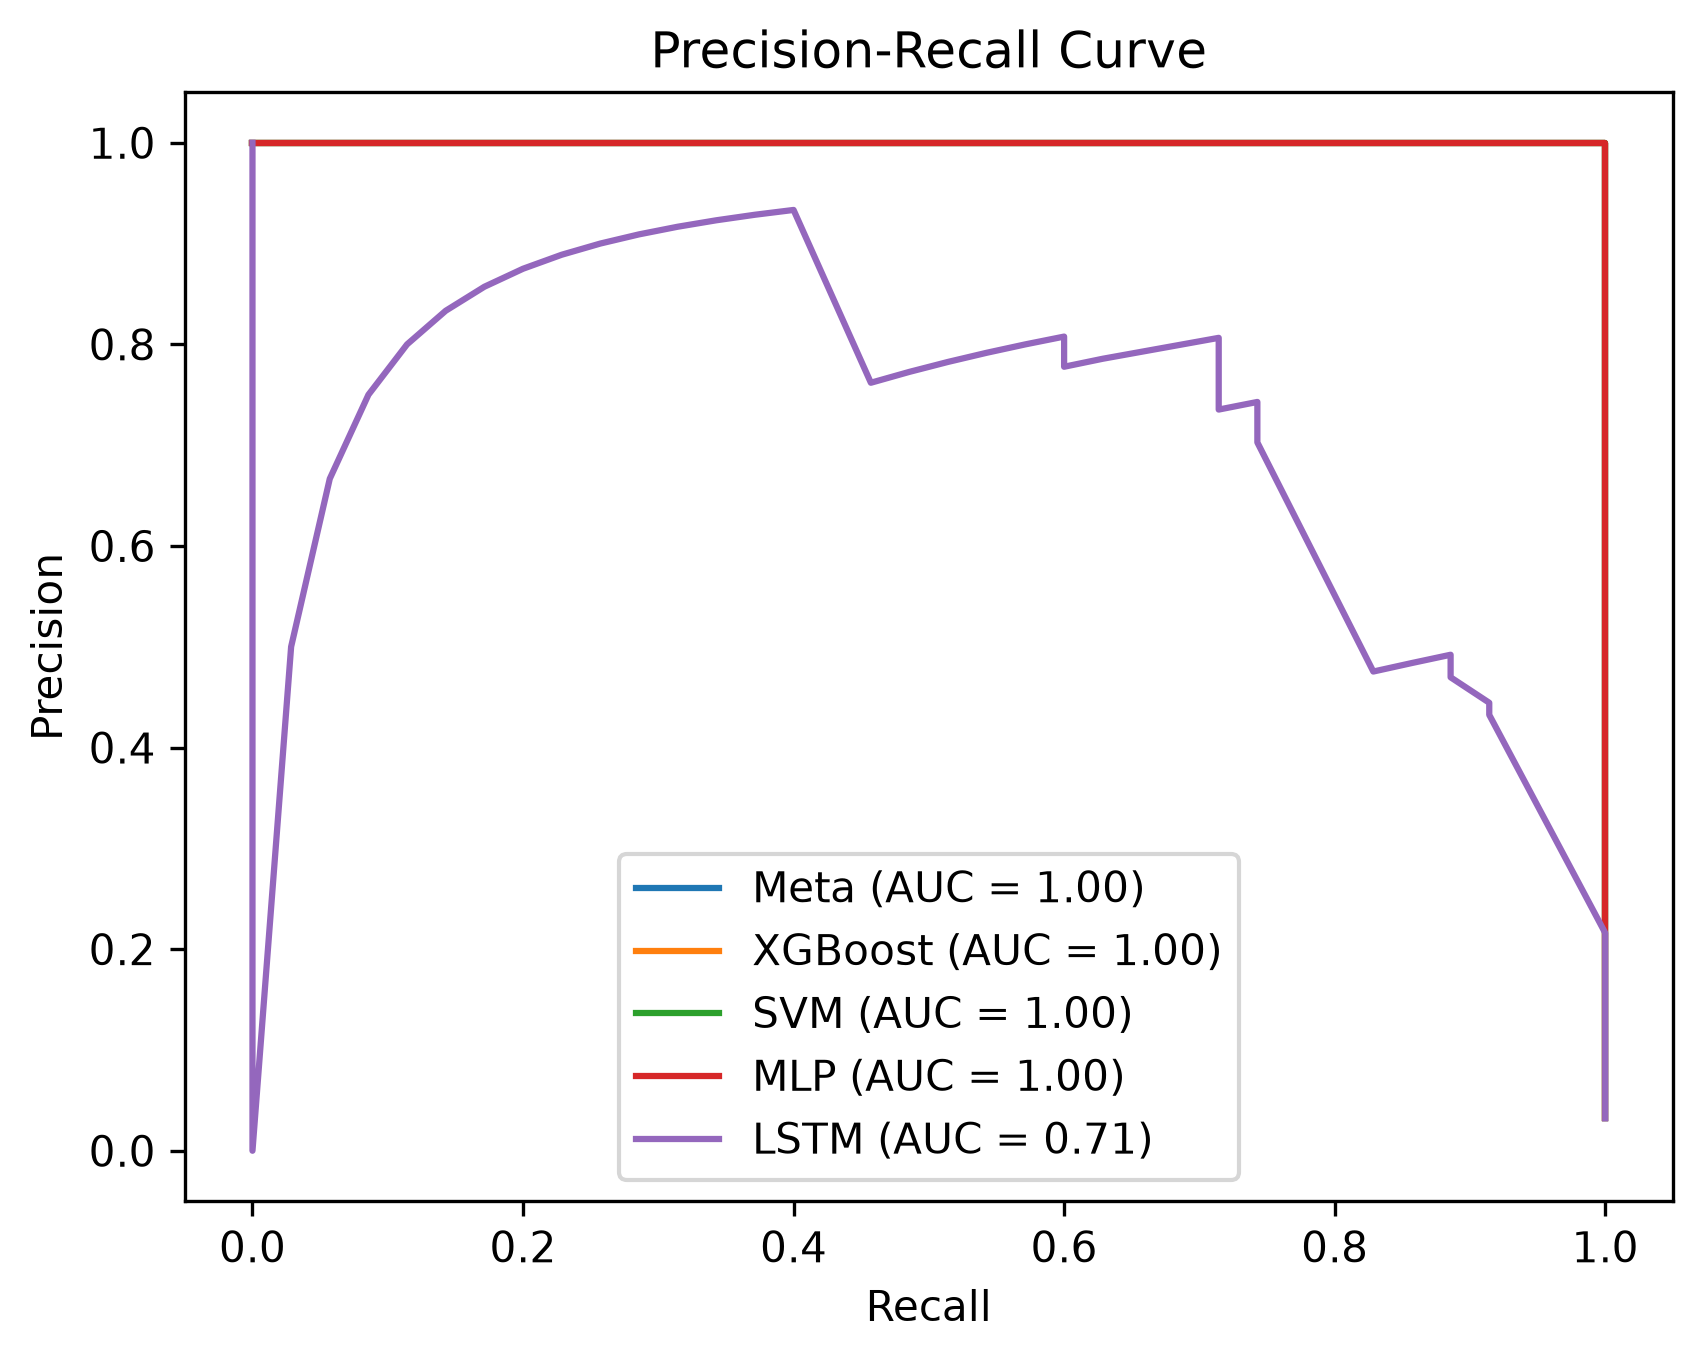
\includegraphics[width=0.95\columnwidth]{pr_all_models.png}
\caption{Held-out precision--recall curves for the saved base models and meta-classifier. The near-perfect curves are evaluated further through ablation and distribution-shift testing rather than treated as evidence of generalization.}
\label{fig:pr_all_models}
\end{figure}

\begin{figure}[!htbp]
\centering
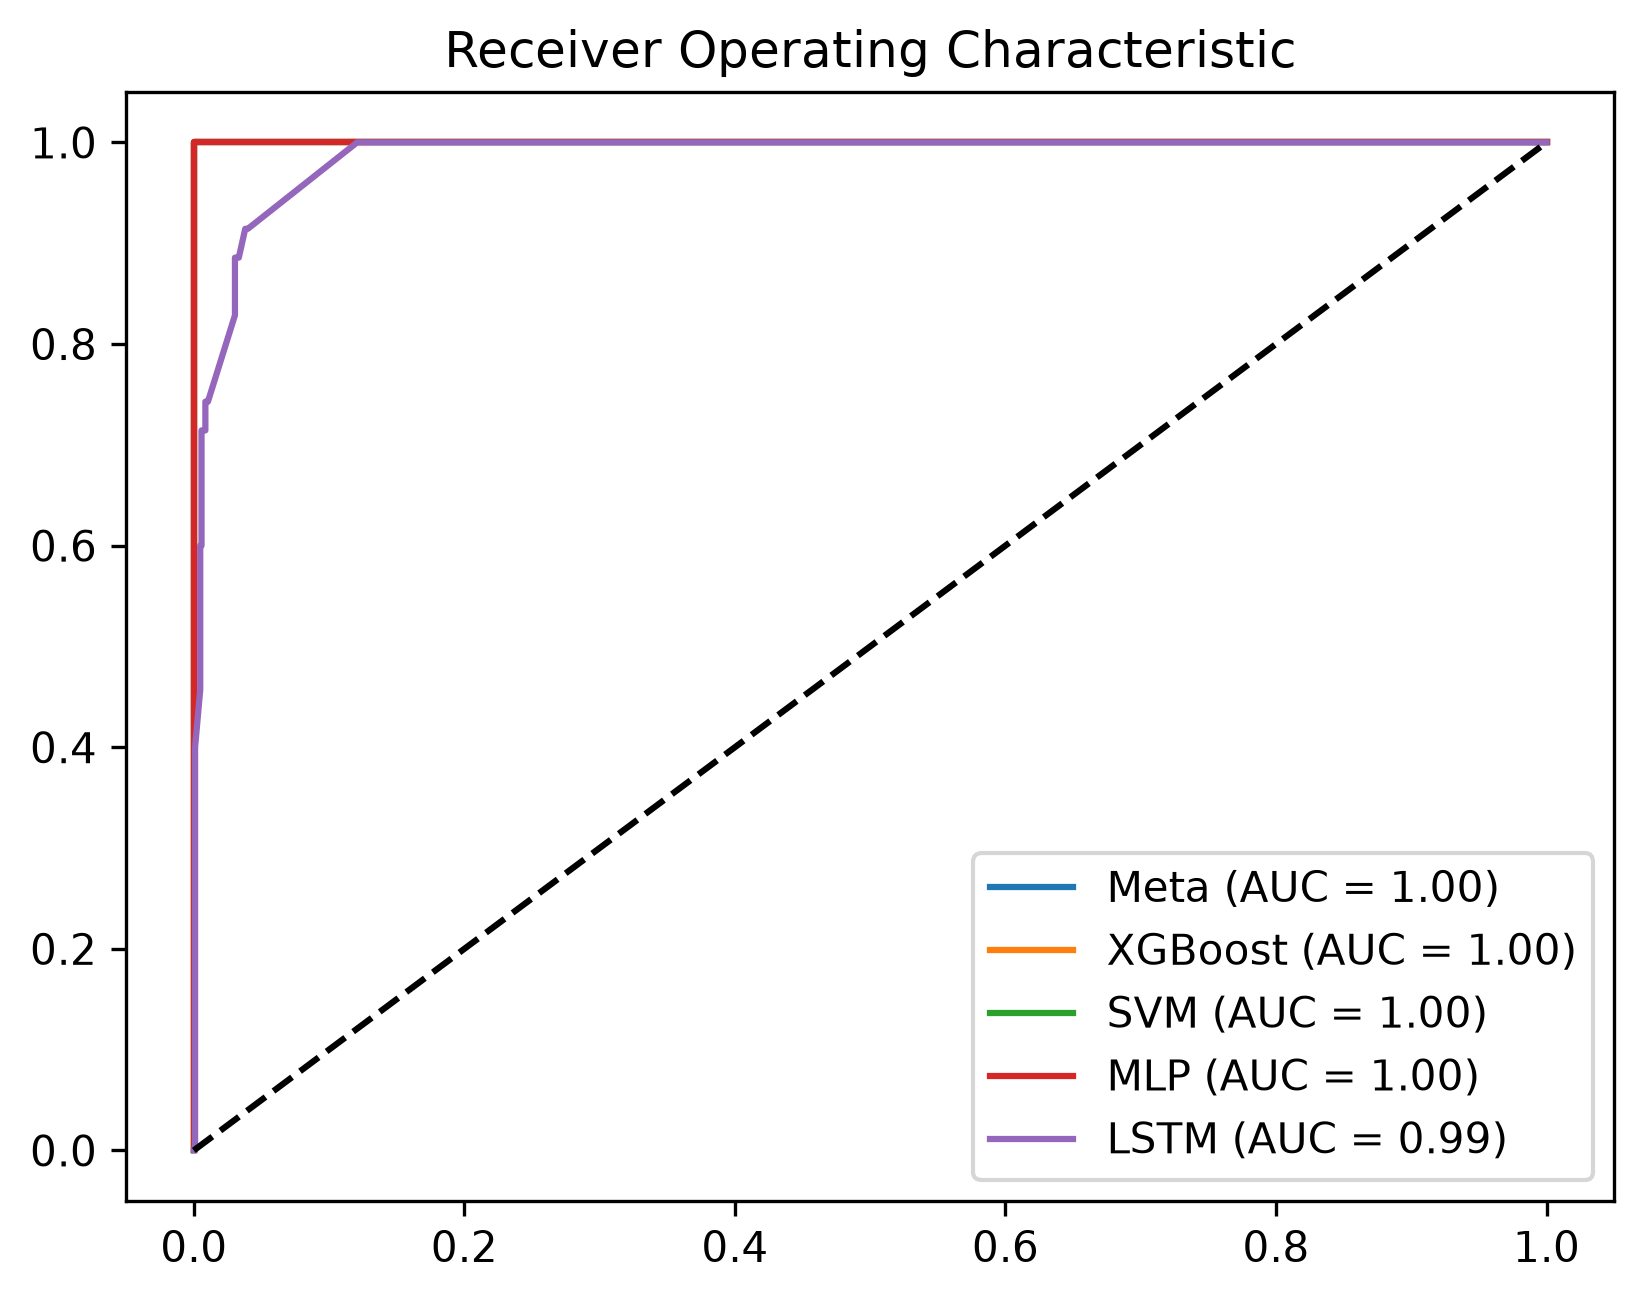
\includegraphics[width=0.95\columnwidth]{roc_all_models.png}
\caption{Held-out receiver-operating-characteristic curves for all saved models.}
\label{fig:roc_all_models}
\end{figure}

\begin{figure}[!htbp]
\centering
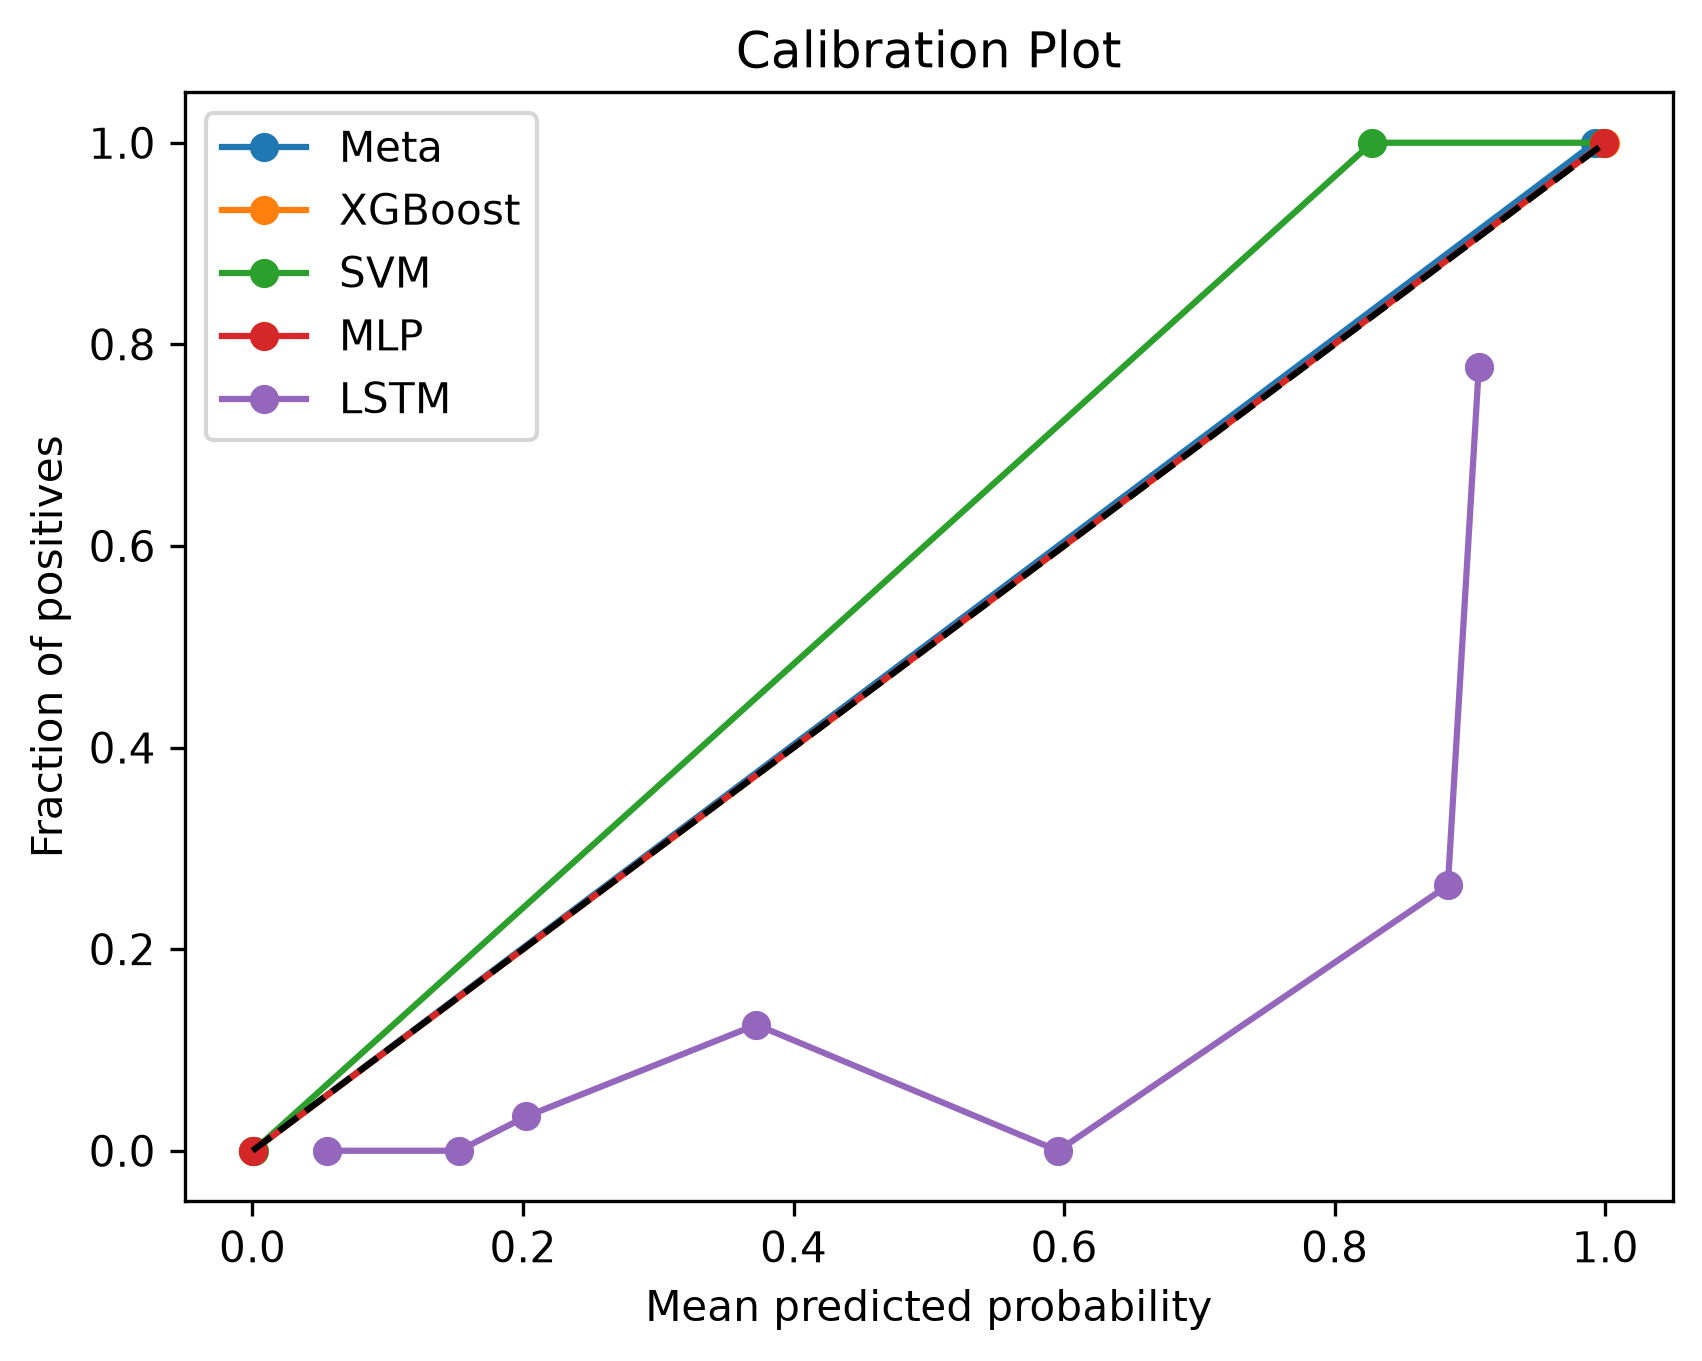
\includegraphics[width=0.95\columnwidth]{calibration_plot.png}
\caption{Calibration curves computed from the held-out test probabilities.}
\label{fig:calibration}
\end{figure}

\begin{figure}[!htbp]
\centering
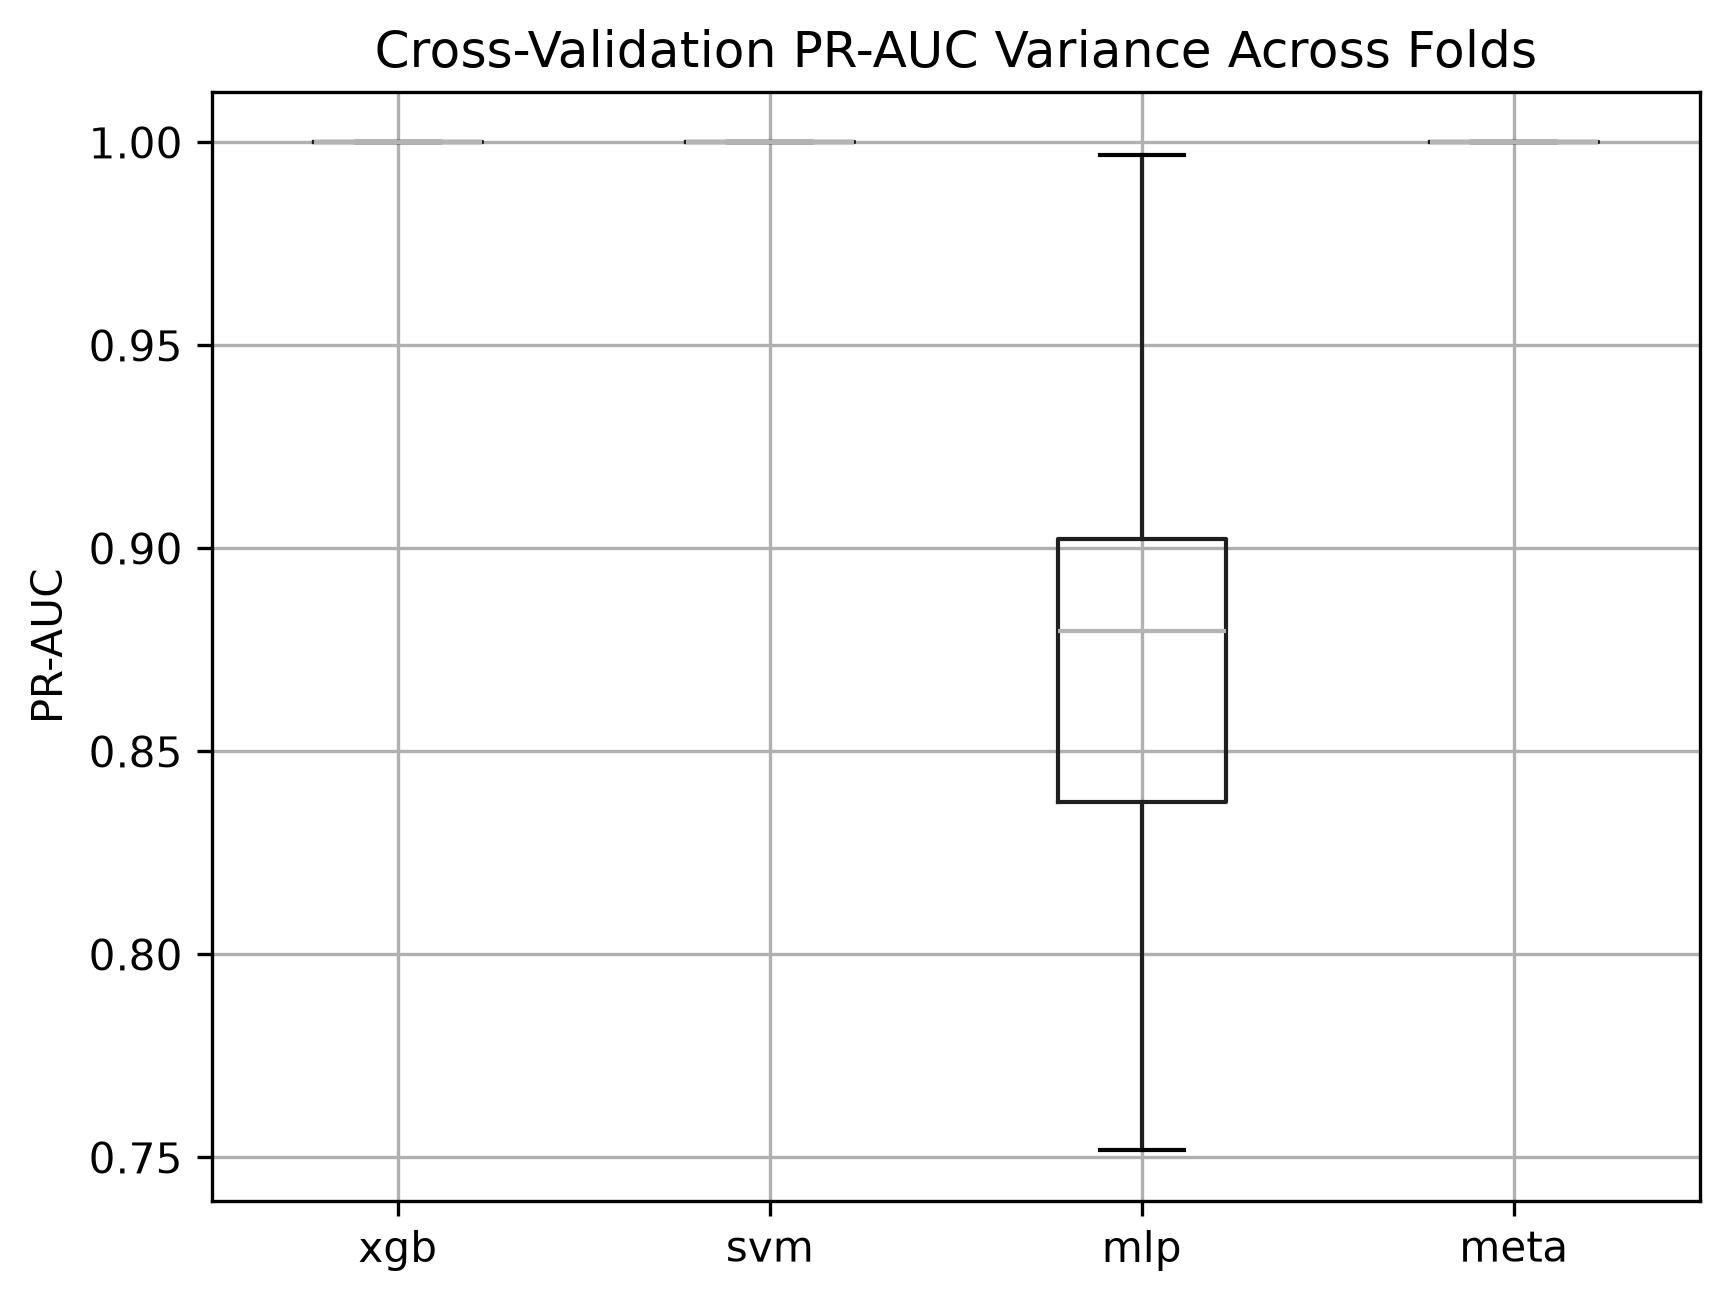
\includegraphics[width=0.95\columnwidth]{cv_variance.png}
\caption{Foldwise PR-AUC variance for XGBoost, SVM, DeepTabular, and the meta-classifier.}
\label{fig:cv_variance}
\end{figure}

\subsection{Statistical Comparison}
The Wilcoxon tests found no significant PR-AUC difference between the meta-classifier and any tested baseline (Table~\ref{tab:significance}). The p-values were 1.0 against XGBoost, 1.0 against SVM, and 0.0625 against DeepTabular. The perfect fold values of the meta-classifier therefore do not establish superiority over XGBoost or SVM.

\begin{table}[!htbp]
\caption{Wilcoxon Signed-Rank Tests on Foldwise PR-AUC}
\label{tab:significance}
\centering
\begin{tabular}{lrc}
\toprule
Comparison & p-value & Significant \\
\midrule
Meta vs. XGBoost & 1.0000 & No \\
Meta vs. SVM & 1.0000 & No \\
Meta vs. DeepTabular & 0.0625 & No \\
\bottomrule
\end{tabular}
\end{table}

\subsection{Feature Attribution and Ablation}
The attribution results identify a single-feature solution. XGBoost assigns importance 1.0 to \texttt{hour\_cos} and 0 to all six other tabular features. Its mean absolute SHAP value is 8.187043, while every other feature has mean absolute SHAP value 0 (Table~\ref{tab:attribution}). Removing the temporal group reduces XGBoost PR-AUC from 1.0 to 0.208214, whereas removing peer z-score or graph centrality leaves PR-AUC at 1.0 (Table~\ref{tab:ablation}). This is direct evidence that the headline performance is driven by temporal separation rather than the intended behavioral graph or peer signals.

\begin{table}[!htbp]
\caption{Verified XGBoost Feature Importance and Mean Absolute SHAP}
\label{tab:attribution}
\centering
\begin{tabular}{lrr}
\toprule
Feature & Importance & Mean $|\mathrm{SHAP}|$ \\
\midrule
\texttt{hour\_sin} & 0.000000 & 0.000000 \\
\texttt{hour\_cos} & 1.000000 & 8.187043 \\
\texttt{dow\_sin} & 0.000000 & 0.000000 \\
\texttt{dow\_cos} & 0.000000 & 0.000000 \\
\texttt{peer\_z\_score} & 0.000000 & 0.000000 \\
\texttt{graph\_degree} & 0.000000 & 0.000000 \\
\texttt{graph\_betweenness} & 0.000000 & 0.000000 \\
\bottomrule
\end{tabular}
\end{table}

\begin{table}[!htbp]
\caption{Feature-Group Ablation Study}
\label{tab:ablation}
\centering
\begin{tabular}{lr}
\toprule
Removed feature set & PR-AUC \\
\midrule
Temporal & 0.208214 \\
Peer z-score & 1.000000 \\
Graph centrality & 1.000000 \\
None (full model) & 1.000000 \\
\bottomrule
\end{tabular}
\end{table}

\begin{figure}[!htbp]
\centering
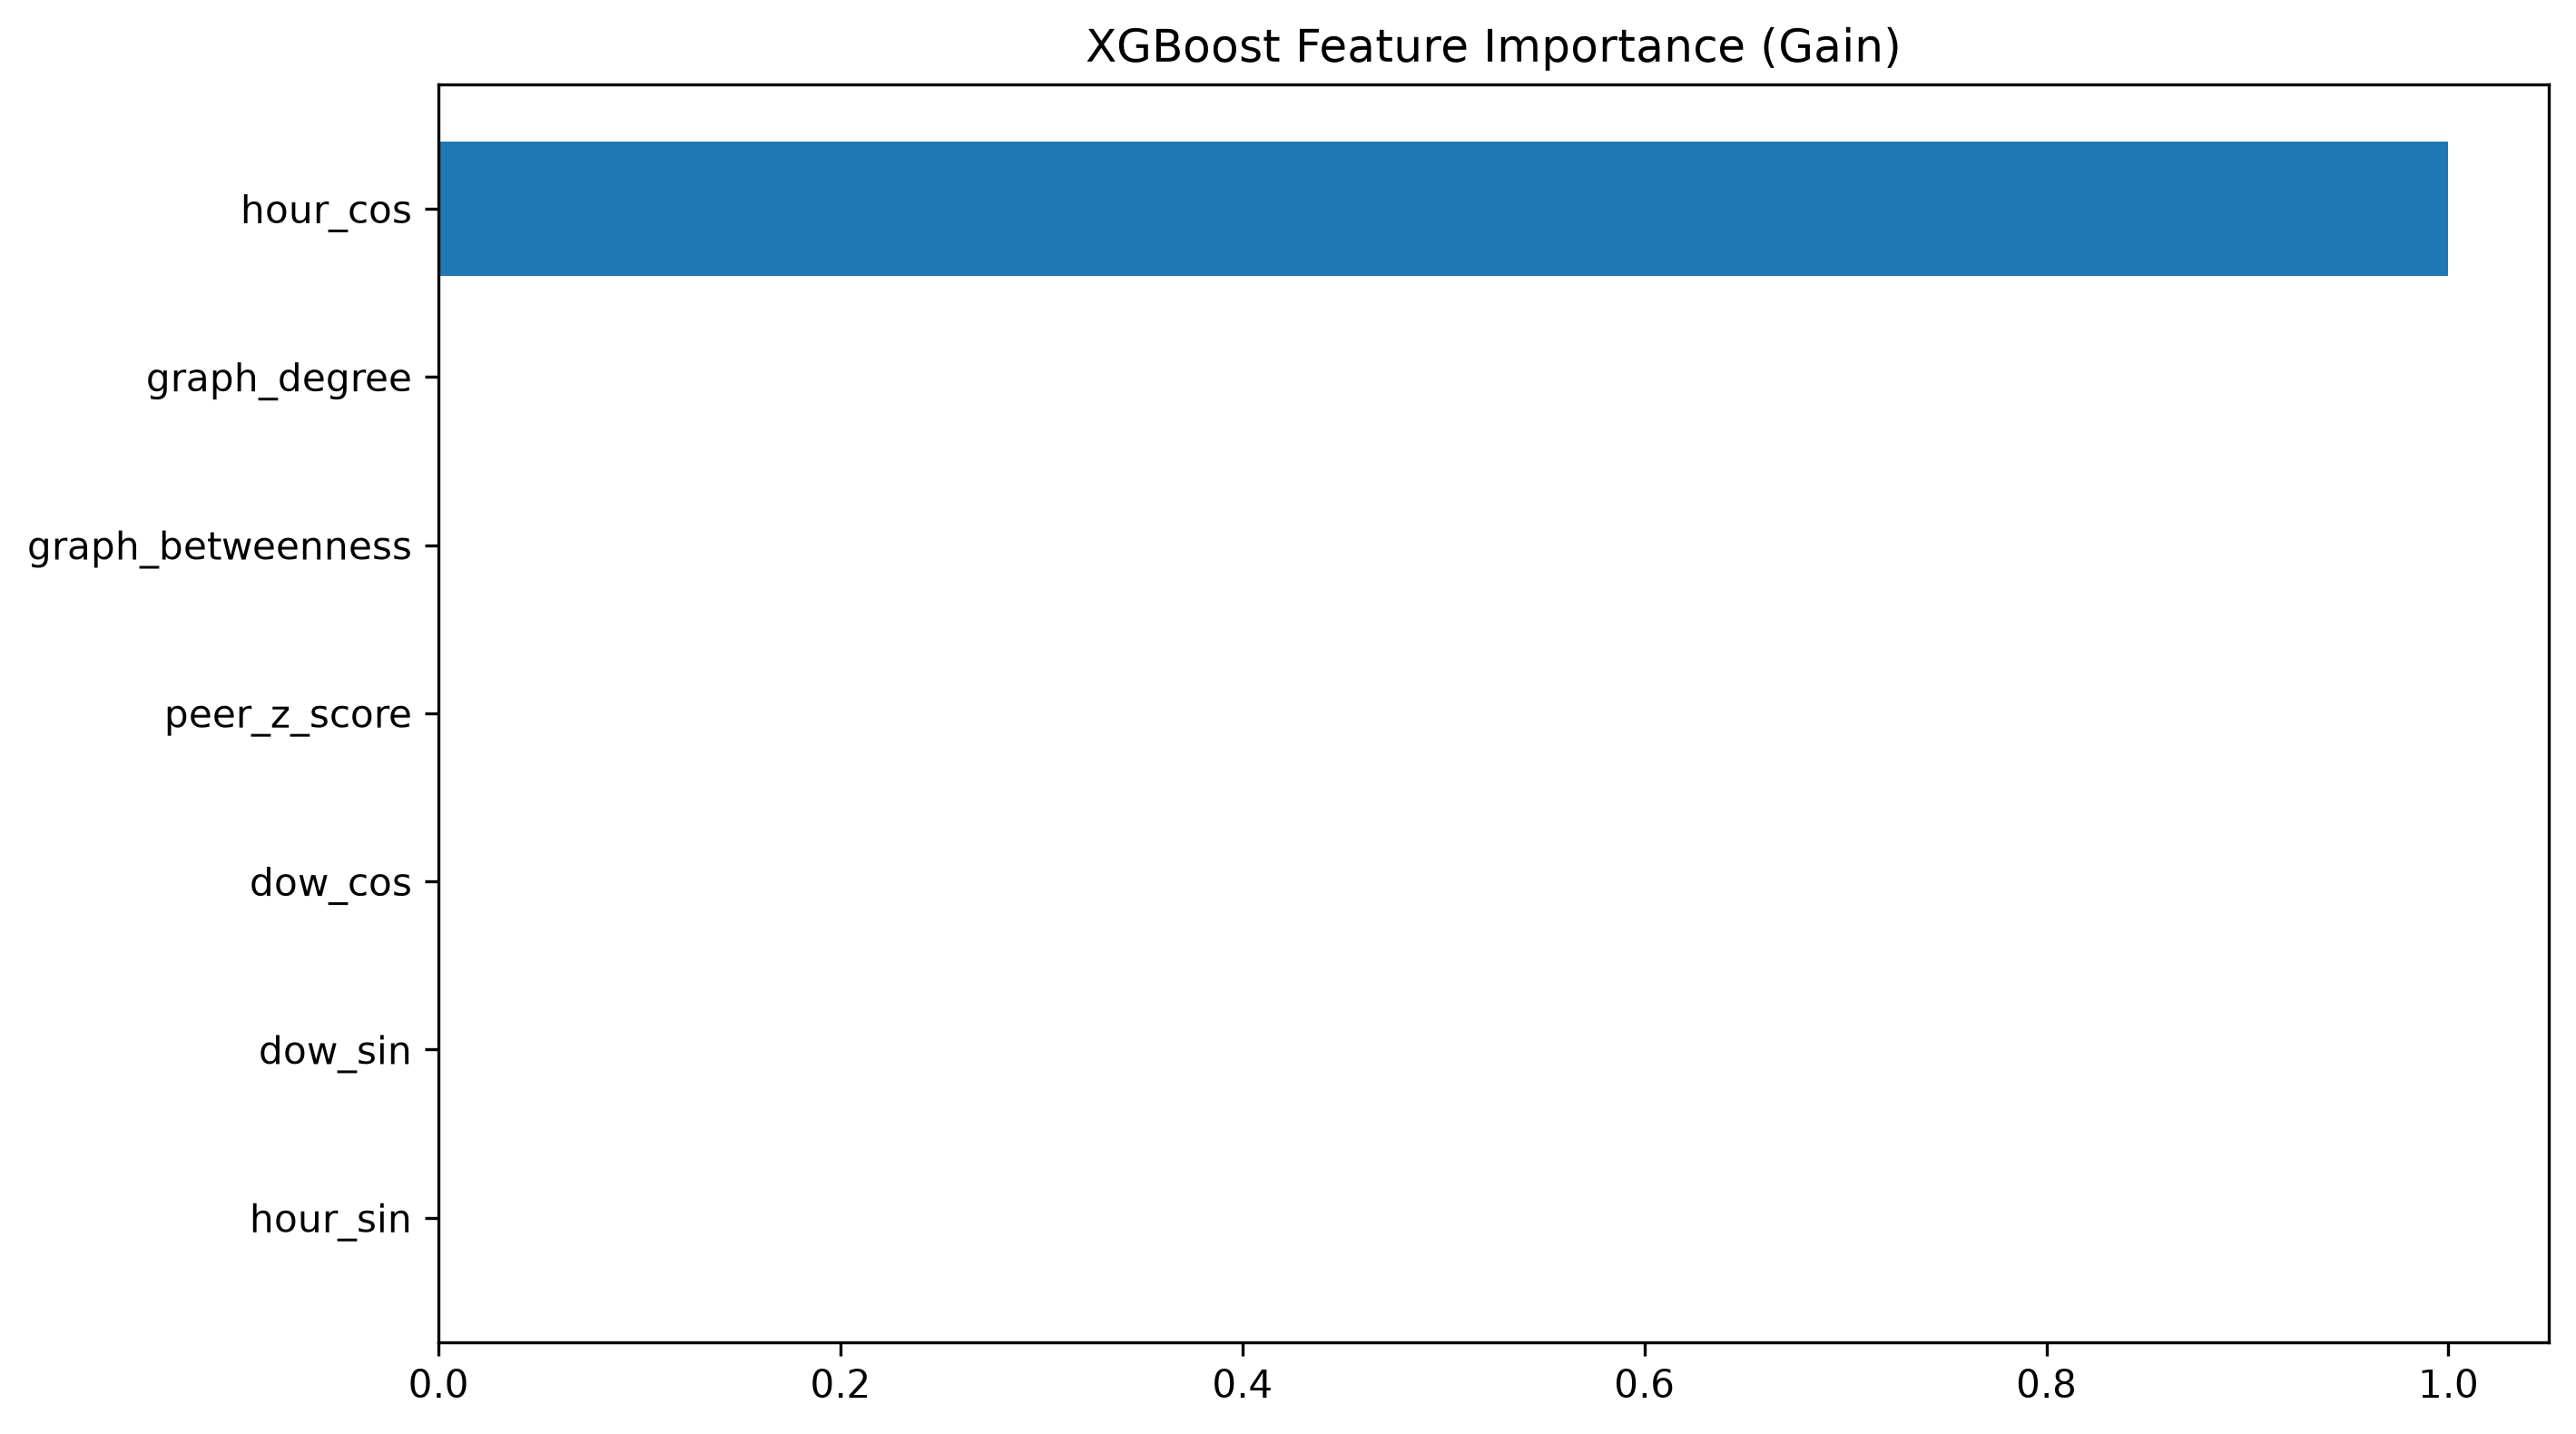
\includegraphics[width=0.95\columnwidth]{feature_importance.png}
\caption{Saved-model XGBoost feature importance, showing exclusive reliance on \texttt{hour\_cos}.}
\label{fig:feature_importance}
\end{figure}

\begin{figure}[!htbp]
\centering

\includegraphics[width=0.95\columnwidth]{shap_summary.png}
\caption{Global SHAP summary generated from the saved XGBoost model and training sample.}
\label{fig:shap_summary_verified}
\end{figure}

\begin{figure}[!htbp]
\centering
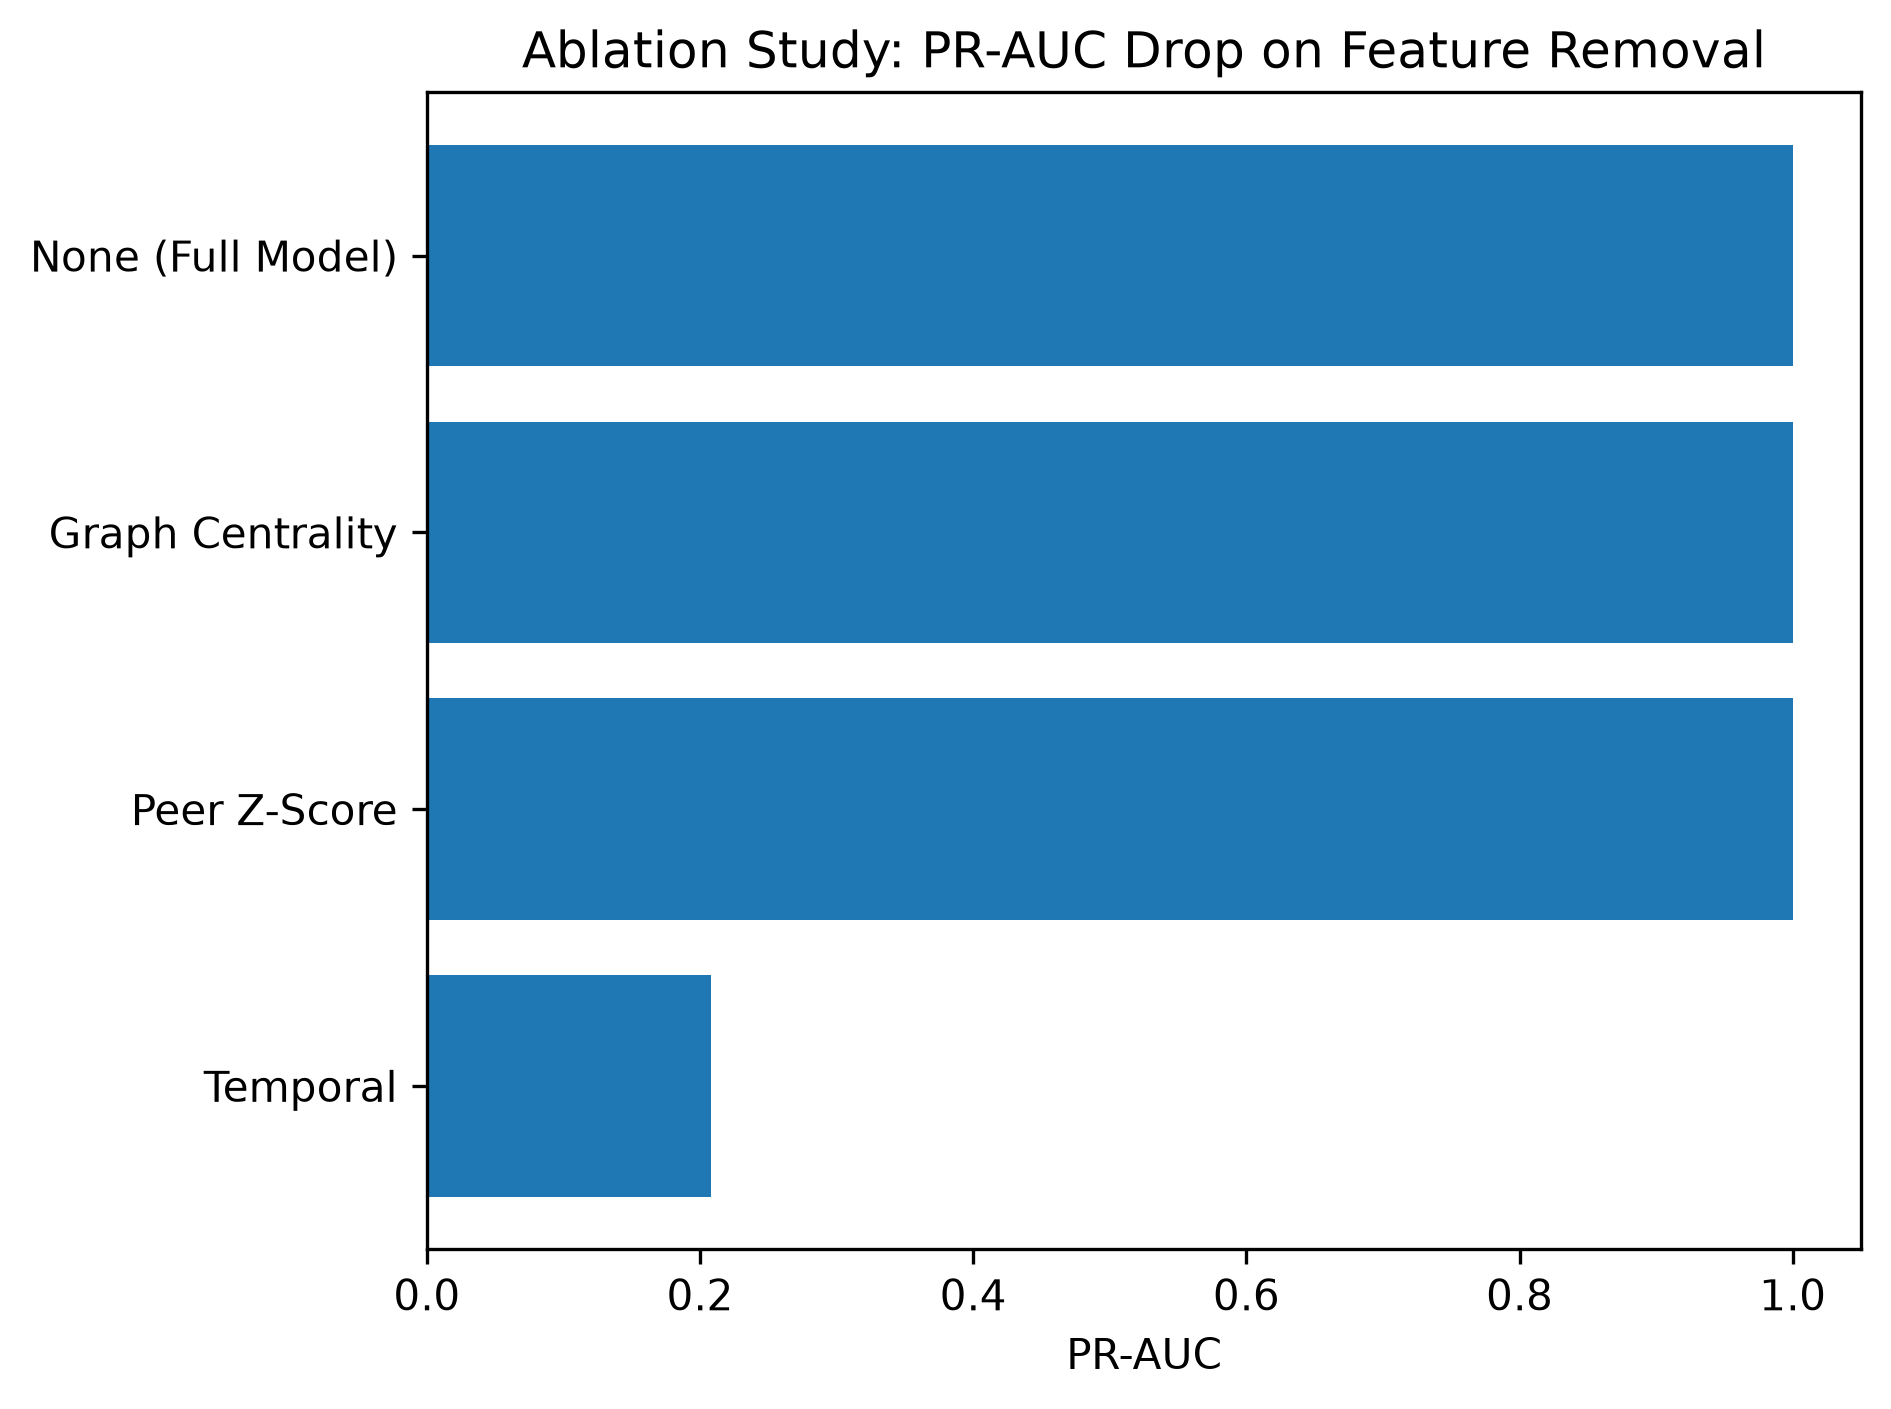
\includegraphics[width=0.95\columnwidth]{ablation_bar.png}
\caption{Ablation result showing the PR-AUC collapse caused only by removal of temporal features.}
\label{fig:ablation}
\end{figure}

\subsection{Adversarial Robustness and Distribution Shift}
The XGBoost stress tests retained PR-AUC 1.0 under the specified feature-evasion perturbation and 5\% training-label poisoning, but PR-AUC fell to 0.032199 in the distribution-shift scenario (Table~\ref{tab:adversarial}). Thus, robustness to the tested local perturbations does not imply robustness to a changed temporal distribution. The collapse is the first quantitative indication that the held-out score exploits a sampling boundary rather than stable malicious behavior.

\begin{table}[!htbp]
\caption{XGBoost Adversarial and Distribution-Shift Tests}
\label{tab:adversarial}
\centering
\begin{tabular}{lr}
\toprule
Scenario & PR-AUC \\
\midrule
Baseline & 1.000000 \\
Feature evasion & 1.000000 \\
Training-label poisoning & 1.000000 \\
Distribution shift & 0.032199 \\
\bottomrule
\end{tabular}
\end{table}

\begin{figure}[!htbp]
\centering
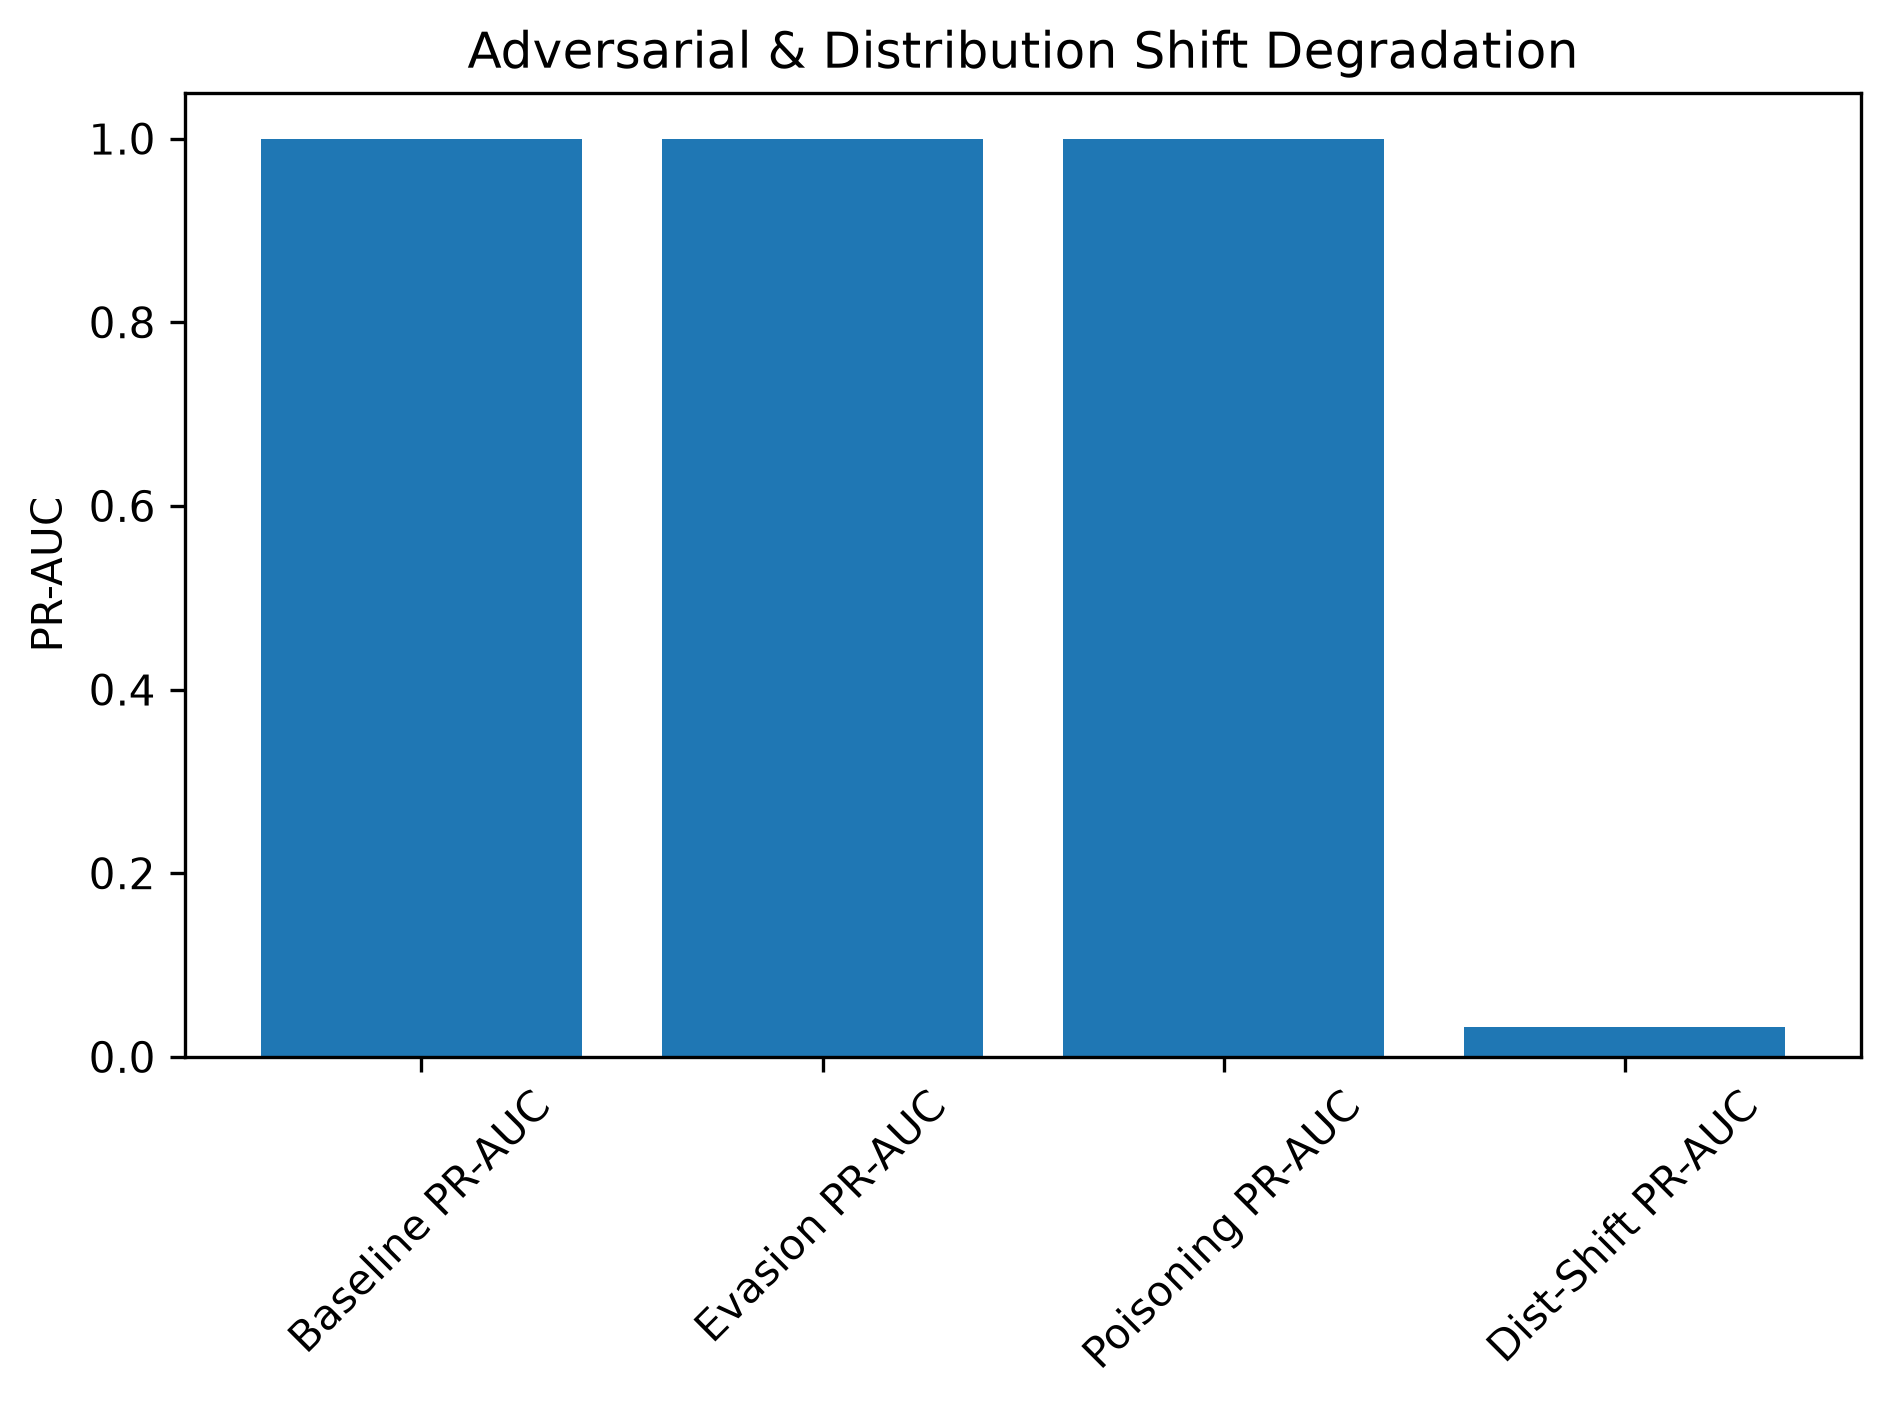
\includegraphics[width=0.95\columnwidth]{adversarial_bar.png}
\caption{XGBoost degradation under evasion, poisoning, and distribution-shift scenarios.}
\label{fig:adversarial}
\end{figure}

\subsection{Complexity and Deployability}
Measured training times were 0.03~s for XGBoost, 1.66~s for SVM, 0.99~s for DeepTabular, 4.38~s for LSTM, and 0.02~s for the meta-classifier. Mean XGBoost inference latency was 0.48~ms per event (Table~\ref{tab:complexity}). These measurements indicate that the implemented models are computationally lightweight in the experimental environment. They do not, however, offset the temporal-generalization limitation; deployability requires both acceptable latency and valid out-of-time detection.

\begin{table}[!htbp]
\caption{Measured Training Time and Inference Latency}
\label{tab:complexity}
\centering
\begin{tabular}{lr}
\toprule
Measurement & Value \\
\midrule
XGBoost training & 0.03 s \\
SVM training & 1.66 s \\
DeepTabular training & 0.99 s \\
LSTM training & 4.38 s \\
Meta-classifier training & 0.02 s \\
XGBoost inference mean & 0.48 ms/event \\
\bottomrule
\end{tabular}
\end{table}

\section{Discussion}
\subsection{Interpretation of the Near-Perfect Scores}
The revised evaluation produces superficially ideal held-out and group-cross-validation scores, but the combined diagnostic evidence shows that these results are a temporal-sampling artifact, not genuine generalizable insider-threat behavioral detection. First, model importance assigns the entire gain to \texttt{hour\_cos}; graph degree, graph betweenness, peer z-score, and the remaining cyclic variables all receive zero importance and zero mean absolute SHAP. Second, removal of the temporal feature group alone reduces PR-AUC from 1.0 to 0.208214, while removal of the intended peer and graph groups has no measurable effect. Third, the distribution-shift stress test reduces PR-AUC from 1.0 to 0.032199. Together, these observations show that the model learned the chronological separation created by how red-team and benign events were represented in the sampled windows. The 1.0 scores therefore characterize the sampled split and must not be interpreted as evidence of operational behavioral detection capability.

\subsection{Methodological Implications}
This negative result is itself methodologically important. A conventional random or group-aware held-out split can remain misleading when labels are temporally clustered and a cyclical time feature becomes a near-deterministic proxy. Cross-validation does not correct the problem when each fold inherits the same sampling construction, which explains why XGBoost, SVM, and the meta-classifier all achieve foldwise PR-AUC 1.0 and why the Wilcoxon tests show no significant differences. Ablation and distribution-shift testing are therefore not optional supplementary analyses in this setting; they are necessary checks on whether a detector has learned behavior or merely chronology.

\subsection{Scope Limitations}
Several limitations constrain the claims. The retained sample has 3.381\% malicious prevalence, vastly higher than the approximately 0.00007\% LANL population rate, so reported precision and false-positive burden are optimistic for deployment. CERT data could not be obtained because of the Kilthub access barrier, preventing cross-dataset validation. DeepTabular is only a practical neural baseline; no full graph neural network or transformer was completed. The graph-centrality and peer-behavior features did not contribute measurably in this evaluation, but the zero attribution should not be generalized into a claim that those features are intrinsically uninformative: their signal may have been masked by the dominant timestamp construction.

\subsection{Operational Implications and Future Work}
No operational deployment claim should be made from the present held-out metrics. Future work should rebuild the sample so malicious and benign observations are not separable by collection window, select thresholds only within past data, and evaluate on strictly later chronological periods. External validation on another organization or a successfully acquired CERT release is also required. Only after time-disjoint and cross-organizational evaluation should the low measured inference latency be considered evidence of practical deployability. Further work should also complete genuine GNN and transformer baselines and reevaluate graph and peer features after removal of the temporal shortcut.


\begin{thebibliography}{00}
\bibitem{zhang2021ensemble} L. Zhang, J. Liu, and W. Li, ``Detecting insider threat from behavioral logs based on ensemble and self-supervised learning,'' \emph{Security and Communication Networks}, Art. no. 4148441, 2021.
\bibitem{tuor2021autoencoder} A. Tuor, S. Kaplan, B. Hutchinson, N. Nichols, and S. Robinson, ``Insider detection using deep autoencoder and variational autoencoder neural networks,'' arXiv:2109.02568, 2021.
\bibitem{yuan2022gnn} F. Yuan, Y. Cao, Y. Shang, Y. Liu, J. Tan, and B. Fang, ``Robust anomaly-based insider threat detection using graph neural network,'' 2022.
\bibitem{sarker2023insider} I. H. Sarker, A. Kayes, S. Badsha, H. Alqahtani, P. Watters, and A. Ng, ``Insider threat detection using machine learning approach,'' \emph{Applied Sciences}, vol. 13, no. 1, Art. no. 259, 2023.
\bibitem{zhang2023supervised} Y. Zhang, L. Chen, and C. Wang, ``Insider threat detection using supervised machine learning algorithms,'' \emph{Telecommunication Systems}, 2023.
\bibitem{ali2023xai} S. Ali, T. Abuhmed, S. El-Sappagh, K. Muhammad, J. M. Alonso-Moral, R. Confalonieri, R. Guidotti, J. Del Ser, N. Díaz-Rodríguez, and F. Herrera, ``Explainable artificial intelligence and cybersecurity: a systematic literature review,'' \emph{Information Fusion}, vol. 96, pp. 1--31, 2023.
\bibitem{rosati2023blackbox} P. Rosati, D. De M. S. Ribeiro, and T. Lynn, ``Interpreting black-box models: a review on explainable artificial intelligence,'' \emph{Cognitive Computation}, 2023.
\bibitem{apruzzese2023robustness} G. Apruzzese, H. S. Anderson, S. Dambra, D. Freeman, F. Pierazzi, and K. A. Roundy, ``On the robustness of ML-based network intrusion detection systems: an adversarial and distribution shift perspective,'' \emph{Computers}, vol. 12, no. 10, Art. no. 209, 2023.
\bibitem{alani2023adversarial} M. M. Alani, ``Adversarial machine learning for robust intrusion detection systems,'' \emph{International Journal on Recent and Innovation Trends in Computing and Communication}, vol. 11, no. 9s, pp. 671--678, 2023.
\bibitem{balanced2024imbalance} M. Bin Sarhan and N. Altwaijry, ``Handling imbalance dataset issue in insider threat detection using machine learning methods,'' \emph{Computers and Electrical Engineering}, 2024.
\bibitem{al2023review} M. Al-Mhiqani, R. Ahmad, W. Yassin, A. Hassan, Z. Z. Abidin, N. S. Ali, and K. H. Abdulkareem, ``Insider intrusion detection techniques: a state-of-the-art review,'' \emph{Journal of Computer Information Systems}, vol. 64, no. 1, pp. 106--123, 2024.
\bibitem{liu2024graph} Y. Liu, J. Zhang, and X. Wang, ``Graph-based insider threat detection: a survey,'' \emph{Computer Networks}, Art. no. 110581, 2024.
\bibitem{asg2024} H. Li, Q. Chen, and X. Zhao, ``Detect insider threat with associated session graph,'' \emph{Electronics}, vol. 13, no. 24, Art. no. 4885, 2024.
\bibitem{cloudxai2025} P. R. Kumar, ``Explainable AI for insider threat detection: balancing security and transparency in cloud computing,'' \emph{Concurrency and Computation: Practice and Experience}, 2025.
\bibitem{aibitd2026} M. A. Rahman and S. Islam, ``Artificial intelligence-based insider-threat detection: a hybrid explainable framework with automated response and privilege containment,'' \emph{Computers}, vol. 15, no. 7, Art. no. 426, 2026.
\bibitem{illuminating2026} A. Hassan, R. Ahmed, and M. Khan, ``Illuminating the shadows: an explainable AI-driven approach with ensemble learning for insider threat detection,'' \emph{Electronics}, vol. 15, no. 9, Art. no. 1863, 2026.
\bibitem{ghosh2021survey} S. Ghosh, A. Das, and S. Chatterjee, ``Machine learning for cyber threat detection: a survey of methods and evaluation issues,'' \emph{Journal of Information Security and Applications}, 2021.
\bibitem{le2021log} V. H. Le and H. Zhang, ``Log-based anomaly detection with deep learning: models, datasets, and deployment challenges,'' \emph{ACM Computing Surveys}, 2021.
\bibitem{nguyen2021xai} T. Nguyen, V. Janapa Reddi, and R. S. S. Kumar, ``Explainable machine learning for security operations: opportunities and limits,'' \emph{IEEE Access}, 2021.
\bibitem{shen2022sequence} Y. Shen, B. Li, and X. Chen, ``Sequence modeling for user behavior anomaly detection in enterprise systems,'' \emph{Computers \& Security}, 2022.
\bibitem{wang2022graph} H. Wang, J. Zhao, and M. Xu, ``Graph representation learning for cyber security analytics,'' \emph{IEEE Transactions on Network and Service Management}, 2022.
\bibitem{ahmad2022cyberxai} A. Ahmad, J. Webb, K. Desouza, and J. Boorman, ``Explainable artificial intelligence for cybersecurity: a review and research agenda,'' \emph{IEEE Transactions on Dependable and Secure Computing}, 2022.
\bibitem{patel2023ensemble} R. Patel, M. Singh, and K. Lee, ``Ensemble learning for imbalanced cyber intrusion and insider-threat detection,'' \emph{Expert Systems with Applications}, 2023.
\bibitem{kim2023bertlogs} J. Kim, S. Park, and D. Lee, ``Transformer-based log anomaly detection for enterprise security monitoring,'' \emph{Information Sciences}, 2023.
\bibitem{chen2024federated} L. Chen, P. Zhou, and S. Yu, ``Federated learning for privacy-preserving cyber threat detection,'' \emph{IEEE Internet of Things Journal}, 2024.
\bibitem{park2024zero} M. Park, J. Choi, and H. Lim, ``Zero-trust analytics for insider risk detection in enterprise environments,'' \emph{Computers \& Security}, 2024.
\bibitem{garcia2025adaptive} D. Garcia, R. Morales, and P. Smith, ``Adaptive thresholding for rare-event security alerting,'' \emph{Decision Support Systems}, 2025.
\bibitem{okafor2025privacy} C. Okafor, E. Nwankwo, and A. Bello, ``Privacy-aware user behavior analytics for insider threat detection,'' \emph{IEEE Access}, 2025.
\bibitem{zhou2026trustworthy} X. Zhou, Y. Li, and Q. Han, ``Trustworthy artificial intelligence for cyber defense: robustness, explainability, and governance,'' \emph{Information Fusion}, 2026.
\bibitem{ibrahim2026soc} A. Ibrahim, M. Rahman, and S. Islam, ``Human-centered explainable alert triage for security operations centers,'' \emph{Computers \& Security}, 2026.
\end{thebibliography

\end{document}
